\chapter{Modello di Scheduling Policy-Driven}
\label{cap:modello}

Il capitolo precedente ha introdotto la struttura astratta del problema, definendo le entità del sistema, le famiglie di politiche $\mathcal{C_A}$, $\mathcal{C_T}$ e $\mathcal{C_D}$, l'insieme degli indicatori $\Phi$ e la funzione di assegnazione $f$, che seleziona il nodo ottimale tra quelli ammissibili mediante la funzione di ottimizzazione $\mathcal{S}_\Phi$. Questi elementi sono stati volutamente presentati in forma generale, rimandandone il contenuto concreto a questo capitolo.

L'obiettivo ora è approfondire ciascuna delle componenti finora introdotte. Si analizza innanzitutto la classificazione dei nodi in base a proprietà astratte, sulla quale si fondano la politica di compatibilità $c_{prop}$ e il relativo indicatore $\phi_{prop}$. Successivamente viene descritto il raggruppamento geografico dei nodi, che costituisce la base della politica di co-locazione $c_{geo}$, seguito dall'introduzione del vincolo di staticità di alcuni dataset, da cui deriva la politica $c_{static}$. Si presenta poi l'indicatore $\phi_{transfer}$ per l'ottimizzazione del trasferimento dei dati remoti. Infine, viene illustrato il modello dei contesti e dei conflitti di interesse, che porta alla definizione della politica di autorizzazione $c_{auth}$ e della politica di isolamento $c_{wall}$ a protezione delle tracce che i dati lasciano sul nodo dopo la loro elaborazione.

% ------------------------------------------------------------ %

\section{Classificazione e Compatibilità delle Proprietà}
\label{sec:classificazione_compatibilita}

Il primo aspetto da approfondire riguarda le proprietà astratte dei nodi e la loro compatibilità con i requisiti dichiarati dalle entità del sistema. Si introduce quindi un meccanismo di classificazione dei nodi rispetto a un insieme di proprietà di alto livello, per poi definire, a partire da questa classificazione, la politica $c_{prop}$ che ne verifica la compatibilità con i requisiti di task e dataset, e l'indicatore $\phi_{prop}$ che ne quantifica la qualità dell'assegnazione.

% ------------------------------------------------------------ %

\subsection{Classificazione dei Nodi}
\label{subsec:classificazione_nodi}

In questa sezione viene introdotto il modello per la classificazione dei nodi del cluster. L'approccio adottato si ispira al modello proposto in~\cite{sec-aware-data-alloc-multicloud} per la classificazione dei servizi cloud in scenari multicloud, adattandolo al contesto di un cluster distribuito in cui i nodi rappresentano le unità di elaborazione dei task. L'idea di fondo è separare le proprietà astratte dei nodi dalla loro descrizione concreta in termini di attributi tecnici: questa separazione consente alle politiche del sistema di fare riferimento a concetti di alto livello, senza dipendere dai dettagli delle configurazioni di ciascun nodo, e permette di definire la corrispondenza tra proprietà e attributi una volta sola in modo centralizzato.

I nodi del cluster sono entità eterogenee: alcuni potrebbero offrire garanzie di sicurezza elevate grazie a specifiche certificazioni e configurazioni di rete, altri si potrebbero distinguere per la capacità di elaborazione disponibile. Un sistema che vuole assegnare i task e gestire i dataset in modo corretto deve poter ragionare su queste differenze in modo sistematico e uniforme. Se si ragionasse direttamente sugli attributi concreti di ciascun nodo all'interno delle politiche ci si scontrerebbe con un approccio meno estendibile e meno flessibile.

Per questo motivo si introduce un livello di astrazione: ogni nodo viene classificato rispetto a un insieme di proprietà astratte, ciascuna delle quali cattura una caratteristica rilevante rispetto alla sua assegnazione, indipendentemente dai dettagli tecnici sottostanti. Le politiche e i requisiti dei task si esprimono quindi in termini di queste proprietà, mentre la corrispondenza con gli attributi concreti resta separata da esse.

Ogni nodo $n \in \mathcal{N}$ del cluster è descritto da un insieme $\mathcal{A}$ di attributi, dove si indica con $n[a]$ il valore dell'attributo $a \in \mathcal{A}$ per il nodo $n$ e con $Dom(a)$ il dominio dei suoi valori. Nella Tabella~\ref{tab:attributi_nodi} è rappresentato un esempio concreto di una possibile struttura dei nodi di un cluster con $\lvert \mathcal{N} \rvert = 5$ e $\mathcal{A} = \{\mathtt{cert},\, \mathtt{isolation},\, \mathtt{gpu},\, \mathtt{cpu\_core}\}$.

\begin{table}[ht]
    \centering
    \begin{tabular}{ccccc}
        \toprule
        \textbf{Nodo} & \texttt{cert} & \texttt{isolation} & \texttt{gpu} & \texttt{cpu\_core} \\
        \midrule
        $n_1$ & \texttt{certA} & \texttt{strict}   & \texttt{a100} & 16 \\
        $n_2$ & \texttt{certB} & \texttt{standard} & \texttt{t4}   & 8  \\
        $n_3$ & \texttt{certC} & \texttt{standard} & \texttt{-}    & 4  \\
        $n_4$ & \texttt{certC} & \texttt{strict}   & \texttt{a100} & 24 \\
        $n_5$ & \texttt{certA} & \texttt{strict}   & \texttt{-}    & 4  \\
        \bottomrule
    \end{tabular}
    \caption{Nodi del cluster nell'esempio ricorrente con i relativi attributi.}
    \label{tab:attributi_nodi}
\end{table}

Adottando la strategia proposta in~\cite{sec-aware-data-alloc-multicloud}, la classificazione dei nodi è definita a partire da un insieme $\mathcal{P}$ di proprietà astratte. A ciascuna proprietà è associato un insieme ordinato di livelli e a ogni livello corrisponde un'espressione booleana sugli attributi del nodo che ne determinerà l'appartenenza. Formalmente:

\begin{definition}[Proprietà astratte dei nodi]
\label{def:proprieta_astratta}
    Dato un insieme $\mathcal{A}$ di attributi, un insieme $\mathcal{P}$ di proprietà astratte è un insieme in cui ogni elemento $p \in \mathcal{P}$ è una coppia $\langle \mathcal{L}_p,\, e_p \rangle$ dove:
    \begin{itemize}
        \item $\mathcal{L}_p = \{0,1,\ldots,l\} \subset \mathbb{N}_0$ è l'insieme dei livelli della proprietà $p$, un intervallo di $\mathbb{N}_0$ che va da $0$ a $l$, estremi inclusi e senza salti, totalmente ordinato dalla relazione $<$;
        \item $e_p : \mathcal{L}_p \rightarrow \mathcal{E}$ è una funzione che associa a ogni livello $l' \in \mathcal{L}_p$ un'espressione booleana base $e_p(l') \in \mathcal{E}$ sugli attributi in $\mathcal{A}$, con $e_p(0) = \mathtt{true}$ per ogni $p \in \mathcal{P}$.
    \end{itemize}
\end{definition}

Il livello $0$ funge da livello di default: la sua espressione è sempre vera e rappresenta l'assenza di requisiti sulla proprietà associata. Livelli superiori corrispondono a condizioni via via sempre più restrittive. 

Nell'esempio ricorrente si considerano due proprietà astratte con $\mathcal{P} = \{S,\, C\}$ e $\mathcal{L}_S = \mathcal{L}_C = \{0,\, 1,\, 2,\, 3\}$: la sicurezza $S$ cattura le garanzie di sicurezza generali offerte dal nodo, mentre la computazione $C$ ne definisce la capacità elaborativa. Le espressioni associate a ciascun livello sono riportate nella Tabella~\ref{tab:proprieta_nodi}.

\begin{table}[ht]
    \centering
    \begin{tabular}{ccp{10cm}}
        \toprule
        \textbf{Proprietà} & \textbf{Livello} & \textbf{Espressione} \\
        \midrule
        \multirow{4}{*}{$S$}
          & $3$ & $(\mathtt{cert=certA} \lor \mathtt{cert=certB}) \land \mathtt{isolation=strict}$ \\
          & $2$ & $\mathtt{cert=certB} \lor \mathtt{isolation=strict}$ \\
          & $1$ & $\mathtt{cert=certC}$ \\
          & $0$ & $\mathtt{true}$ \\
        \midrule
        \multirow{4}{*}{$C$}
          & $3$ & $(\mathtt{gpu=a100} \lor \mathtt{gpu=h100}) \land \mathtt{cpu\_core \geq 16}$ \\
          & $2$ & $\mathtt{gpu=t4} \lor \mathtt{cpu\_core \geq 8}$ \\
          & $1$ & $\mathtt{cpu\_core \geq 4}$ \\
          & $0$ & $\mathtt{true}$ \\
        \bottomrule
    \end{tabular}
    \caption{Proprietà astratte $S$ e $C$ nell'esempio ricorrente, con le espressioni booleane associate a ciascun livello.}
    \label{tab:proprieta_nodi}
\end{table}

Per la proprietà $S$, il livello 3 richiede isolamento \texttt{strict} e una certificazione elevata, ovvero \texttt{certA} oppure \texttt{certB}. Il livello 2 include invece i nodi che soddisfano almeno una tra la presenza di certificazione \texttt{certB} e l'isolamento \texttt{strict}. Il livello 1 cattura i nodi con certificazione \texttt{certC}. Per la proprietà $C$ invece, il livello 3 è raggiunto dai nodi dotati di acceleratori di fascia alta (come \texttt{a100} o \texttt{h100}) e con almeno 16 core CPU. Il livello 2 include nodi con GPU di fascia intermedia (ad esempio \texttt{t4}) oppure con almeno 8 core CPU. Il livello 1 cattura i nodi con almeno 4 core CPU, indipendentemente dalla presenza di GPU. In entrambi i casi, il livello $0$, come accennato sopra, rappresenta l'assenza di vincoli.

Inoltre, è utile osservare che le espressioni $e_p(l)$ dei livelli $l \in \mathcal{L}_p$ possono teoricamente assumere qualsiasi forma della logica proposizionale sugli attributi, ma adottare una rappresentazione uniforme ne semplificherebbe la specifica e la valutazione nell'implementazione concreta del sistema che sarà discussa al Capitolo~\ref{cap:implementazione}.

Poiché è dimostrato che ogni formula della logica proposizionale può essere riscritta in una forma normale disgiuntiva (DNF, \emph{Disjunctive Normal Form}) equivalente~\cite{prop-logic-dnf}, ogni espressione $e_p(l)$ con $l \in \mathcal{L}_p$ può essere rappresentata senza perdita di generalità come disgiunzione di congiunzioni di condizioni sugli attributi $\mathcal{A}$ di un nodo $n \in \mathcal{N}$:
\begin{equation}
    e_p(l) \equiv \bigvee_{i=1}^{m} \left( \bigwedge_{j=1}^{k_i} \varphi_{i,\,j} \right)
\end{equation}
dove ciascun $\varphi_{i,\,j}$ è una condizione elementare di uno dei seguenti tipi: una condizione di confronto $n[a] \odot v$, con $a \in \mathcal{A}$, $v \in Dom(a)$ e $\odot \in \{=,\, \neq,\, \leq,\, \geq,\, \in,\, \notin,\, \ldots\}$, oppure una condizione di esistenza $\exists\, n[a]$ o di assenza $\nexists\, n[a]$, che verificano rispettivamente la presenza o l'assenza dell'attributo $a$ nel nodo $n$, indipendentemente dal suo valore.

Questa struttura ha un'interpretazione pratica naturale: ogni clausola $\bigwedge_{j} \varphi_{i,\,j}$ della disgiunzione rappresenta una configurazione di attributi sufficiente a qualificare il nodo per un certo livello, e il nodo soddisfa l'espressione se corrisponde ad almeno una di queste configurazioni. Ad esempio, l'espressione del livello 3 della proprietà $C$ dell'esempio ricorrente in forma normale disgiuntiva diventerebbe: 
\begin{equation}
    (\mathtt{gpu=a100} \land \mathtt{cpu\_core} \geq 16) \lor (\mathtt{gpu=h100} \land \mathtt{cpu\_core} \geq 16)
\end{equation}

È immediato osservare che la disgiunzione di un numero finito di formule in DNF produce ancora una formula in DNF. Infatti, date due formule in forma DNF:
\begin{equation}
    e_1 = \bigvee_{i=1}^{m} A_i \qquad e_2 = \bigvee_{j=1}^{h} B_j
\end{equation}
dove ogni $A_i$ e $B_j$ è una congiunzione di condizioni elementari, la loro disgiunzione:
\begin{equation}
    e_1 \lor e_2 
    = \left( \bigvee_{i=1}^{m} A_i \right) \lor \left( \bigvee_{j=1}^{h} B_j \right)
    = \bigvee_{k=1}^{m+h} C_k
\end{equation}
risulta essere sempre in forma DNF, dove $\{C_k\}_{1 \leq k \leq m + h}$ è la famiglia di tutte le clausole di $e_1$ e di $e_2$, ciascuna ancora una congiunzione di condizioni elementari.

Questo risultato consente di definire le espressioni associate a ciascun livello in modo che sia garantita la monotonia dei livelli. L'idea è che l'espressione effettiva al livello $l$ incorpori, in disgiunzione, le espressioni di tutti i livelli superiori. Così se un nodo soddisfa l'espressione di un qualsiasi livello $l' \geq l$, soddisferà automaticamente anche quella del livello $l$.

\begin{definition}[Espressioni effettive dei livelli]
    \label{def:espressioni_effettive}
    Dato un insieme $\mathcal{P}$ di proprietà e, per ogni $p \in \mathcal{P}$, l'insieme di espressioni base $\{e_p(l)\}_{l \in \mathcal{L}_p}$, si definiscono le espressioni effettive $\hat{e}_p : \mathcal{L}_p \rightarrow \mathcal{E}$ come:
    \begin{equation}
        \hat{e}_p(l) = \bigvee_{i = l}^{\max \mathcal{L}_p} e_p(i) 
        \qquad 
        \forall\, l \in \mathcal{L}_p
    \end{equation}
    dove $\max \mathcal{L}_p$ è il livello massimo raggiungibile in $\mathcal{L}_p$. Poiché ciascuna espressione base $e_p(l)$ è in forma DNF, anche ogni espressione effettiva $\hat{e}_p(l)$ risulta espressa in forma DNF.
\end{definition}

Questa risulta essere una scelta di progettazione logica: un nodo che come da esempio soddisfa un certo livello di sicurezza o di computazione, è ragionevole che soddisfi anche i livelli inferiori in una relazione d'ordine totale, i quali esprimono requisiti meno stringenti.

Riprendendo l'esempio ricorrente, le espressioni effettive della proprietà $C$ 
risulteranno quindi:
\begin{align}
    \hat{e}_C(3) &= (\mathtt{gpu=a100} \land \mathtt{cpu\_core} \geq 16) \\
                 \notag &\quad \lor (\mathtt{gpu=h100} \land \mathtt{cpu\_core} \geq 16) \\[1ex]
    \hat{e}_C(2) &= (\mathtt{gpu=t4}) \lor (\mathtt{cpu\_core} \geq 8) \\
                 \notag &\quad \lor (\mathtt{gpu=a100} \land \mathtt{cpu\_core} \geq 16) \\
                 \notag &\quad \lor (\mathtt{gpu=h100} \land \mathtt{cpu\_core} \geq 16) \\[1ex]
    \hat{e}_C(1) &= (\mathtt{cpu\_core} \geq 4) \\
                 \notag &\quad \lor (\mathtt{gpu=t4}) \lor (\mathtt{cpu\_core} \geq 8) \\
                 \notag &\quad \lor (\mathtt{gpu=a100} \land \mathtt{cpu\_core} \geq 16) \\
                 \notag &\quad \lor (\mathtt{gpu=h100} \land \mathtt{cpu\_core} \geq 16)
\end{align}
Si può facilmente verificare che un nodo con $\mathtt{gpu=a100}$ e $\mathtt{cpu\_core} = 16$ soddisfa $\hat{e}_C(3)$, e per costruzione soddisfa anche $\hat{e}_C(2)$ e $\hat{e}_C(1)$, poiché le clausole di $\hat{e}_C(3)$ sono incluse in entrambe.

Per semplicità, d'ora in avanti verrà indicato con $n \models e$ il fatto che un nodo $n \in \mathcal{N}$ soddisfi l'espressione $e \in \mathcal{E}$. Dunque, la monotonia dei livelli non sarà un'assunzione da imporre esternamente, ma una conseguenza diretta della costruzione delle espressioni effettive.

\begin{theorem}[Monotonia dei livelli delle proprietà]
    \label{teo:monotonia_livelli}
    Per ogni proprietà $p \in \mathcal{P}$, gli insiemi dei nodi che soddisfano i livelli sono annidati rispetto al loro ordine. In particolare, per ogni coppia di livelli $l,\, l' \in \mathcal{L}_p$ tali che $l \geq l'$ vale:
    \begin{equation}
        \left\{ n \in \mathcal{N} \mid n \models \hat{e}_p(l) \right\} 
        \subseteq 
        \left\{ n \in \mathcal{N} \mid n \models \hat{e}_p(l') \right\}
    \end{equation}
    In altre parole, definendo $\mathcal{N}_{p,\,l} = \left\{n \in \mathcal{N} \mid n \models \hat{e}_p(l) \right\}$, la famiglia $\left\{\mathcal{N}_{p,\,l}\right\}_{l \in \mathcal{L}_p}$ forma una catena rispetto ai livelli della proprietà $p$, ossia: 
    \begin{equation}
        \mathcal{N}_{p,\,l} \subseteq \mathcal{N}_{p,\,l-1} 
        \qquad 
        \forall\, l \in \mathcal{L}_p,\; l \geq 1
    \end{equation}
    \begin{proof}
        Siano $l,\, l' \in \mathcal{L}_p$ due livelli tali che $l \geq l'$. Dalla Definizione~\ref{def:espressioni_effettive}, l'espressione effettiva $\hat{e}_p(l)$ si ottiene unendo in disgiunzione i livelli di $p$ da $l$ a $\max \mathcal{L}_p$. Possiamo quindi riscrivere $\hat{e}_p(l')$ come segue:
        \begin{equation}
            \hat{e}_p(l') = \left( \bigvee_{i=l'}^{l-1} e_p(i) \right) \lor \hat{e}_p(l)
        \end{equation}
        Per le regole elementari della logica proposizionale si ha $\hat{e}_p(l) \implies \hat{e}_p(l')$, di conseguenza $n \models \hat{e}_p(l) \implies n \models \hat{e}_p(l')$, da cui segue immediatamente:
        \begin{equation}
            \left\{ n \in \mathcal{N} \mid n \models \hat{e}_p(l) \right\} \subseteq \left\{ n \in \mathcal{N} \mid n \models \hat{e}_p(l') \right\}
        \end{equation}
    \end{proof}
\end{theorem}

Questo significa che, data una proprietà $p \in \mathcal{P}$, se un nodo soddisfa il livello $l \in \mathcal{L}_p$, allora di conseguenza soddisferà tutti i suoi livelli inferiori $l' \in \mathcal{L}_p$ con $l \geq l'$.

\begin{corollary}[Implicazione per soddisfacibilità]
    \label{cor:implicazione_livelli}
    Per ogni nodo $n \in \mathcal{N}$, proprietà $p \in \mathcal{P}$ e livelli $l \geq l'$ in $\mathcal{L}_p$:
    \begin{equation}
        n \models \hat{e}_p(l) \implies n \models \hat{e}_p(l')
    \end{equation}
\end{corollary}

Ai fini della classificazione, il livello di un nodo rispetto a una determinata proprietà sarà dunque definito prendendo in considerazione il massimo tra i livelli soddisfatti.

\begin{definition}[Livello di un nodo rispetto a una proprietà]
    \label{def:livello_nodo}
    Dato un nodo $n \in \mathcal{N}$ e una proprietà $p \in \mathcal{P}$, il livello di $n$ rispetto alla proprietà $p$ è definito da $\alpha_p : \mathcal{N} \rightarrow \mathcal{L}_p$ tale che:
    \begin{equation}
        \alpha_p(n) = \max \left\{ l \in \mathcal{L}_p \mid n \models \hat{e}_p(l) \right\}
    \end{equation}
\end{definition}

È banale dimostrare che il massimo è sempre definito e unico, poiché $e_p(0) = \mathtt{true}$ per ogni proprietà $p \in \mathcal{P}$ garantisce che il livello $0$ appartenga sempre all'insieme dei livelli soddisfatti dal nodo, che risulta quindi non vuoto e, essendo un sottoinsieme finito di $\mathcal{L}_p$, ammette massimo. 

Da questa definizione e dal Teorema~\ref{teo:monotonia_livelli} della monotonia dei livelli delle proprietà segue immediatamente un fatto che semplificherà la verifica delle politiche inerenti alle proprietà dei nodi.

\begin{theorem}[Soddisfacibilità tramite livelli]
    \label{teo:soddisfacibilita_livelli}
    Per ogni nodo $n \in \mathcal{N}$, proprietà $p \in \mathcal{P}$ e livello $l \in \mathcal{L}_p$, sia $\mathcal{N}_{p,\,l} = \{ n \in \mathcal{N} \mid n \models \hat{e}_p(l) \}$ l'insieme dei nodi che soddisfano il livello $l$. Allora vale:
    \begin{equation}
        \alpha_p(n) \geq l \iff n \in \mathcal{N}_{p,\,l}
    \end{equation}

    \begin{proof}
        ($\Rightarrow$) Se $\alpha_p(n) \geq l$, allora per la Definizione~\ref{def:livello_nodo} di $\alpha_p(n)$ esiste un livello $l^* \geq l$ tale che $n \in \mathcal{N}_{p,l^*}$. Dal Teorema~\ref{teo:monotonia_livelli} segue che $\mathcal{N}_{p,l^*} \subseteq \mathcal{N}_{p,l}$, quindi $n \in \mathcal{N}_{p,l}$.
        
        ($\Leftarrow$) Se $n \in \mathcal{N}_{p,l}$, per la Definizione~\ref{def:livello_nodo} di $\alpha_p(n)$ come massimo livello soddisfatto, segue che $\alpha_p(n) \geq l$.
    \end{proof}
\end{theorem}

Il Teorema~\ref{teo:soddisfacibilita_livelli} mostra che il valore $\alpha_p(n)$ rappresenta in modo completo la soddisfacibilità dei livelli associati alla proprietà $p$. In particolare, un nodo soddisfa esattamente tutti e soli i livelli minori o uguali al valore $\alpha_p(n)$. 

Ad esempio, si consideri il nodo $n_1$ della Tabella~\ref{tab:attributi_nodi}. Per la proprietà di sicurezza $S$, il nodo soddisfa il livello massimo $3$, quindi $\alpha_S(n_1) = 3$ e dunque $n_1 \in \mathcal{N}_{S,3}$. Inoltre, per il teorema appena enunciato, segue immediatamente che $n_1 \in \mathcal{N}_{S,\,i}$ con $i \in \{0,\, 1,\, 2\}$. Quindi, invece di rivalutare le espressioni booleane sugli attributi per ogni livello, è sufficiente conoscere il singolo valore $\alpha_S(n_1)$.

In questo modo, un problema inizialmente espresso in termini di condizioni logiche sugli attributi dei nodi viene ricondotto a un confronto tra livelli ordinati. Questo rende la valutazione delle politiche inerenti alle proprietà dei nodi non solo più efficiente, ma anche più semplice da interpretare e implementare. Ora è utile raccogliere in un'unica struttura il livello raggiunto da un nodo per ciascuna proprietà, ovvero la sua classe di proprietà.

\begin{definition}[Classe di proprietà di un nodo]
    \label{def:classe_nodo}
    Dato un insieme di proprietà astratte $\mathcal{P} = \{p_1,\, \ldots,\, p_m\}$, sia $\Gamma = \mathcal{L}_{p_1} \times \ldots \times \mathcal{L}_{p_m}$. La classe di proprietà di un nodo $n \in \mathcal{N}$ è il vettore dato da $\alpha : \mathcal{N} \rightarrow \Gamma$ tale che:
    \begin{equation}
        \alpha(n) = \left[ \alpha_p(n) \right]_{p \in \mathcal{P}}
    \end{equation}
\end{definition}

Applicando le definizioni dei livelli e delle classi di proprietà appena enunciate ai nodi di esempio della Tabella~\ref{tab:attributi_nodi}, con l'insieme di proprietà $\mathcal{P} = \{S,\, C\}$ dell'esempio ricorrente, si ottengono le classi riportate nella Tabella~\ref{tab:classi_nodi}.

\begin{table}[ht]
    \centering
    \begin{tabular}{cccc}
        \toprule
        \textbf{Nodo} & $\alpha_S(n)$ & $\alpha_C(n)$ & $\alpha(n)$ \\
        \midrule
        $n_1$ & 3 & 3 & $[3,\,3]$ \\
        $n_2$ & 2 & 2 & $[2,\,2]$ \\
        $n_3$ & 1 & 1 & $[1,\,1]$ \\
        $n_4$ & 2 & 3 & $[2,\,3]$ \\
        $n_5$ & 3 & 1 & $[3,\,1]$ \\
        \bottomrule
    \end{tabular}
    \caption{Classi di proprietà dei nodi dell'esempio ricorrente.}
    \label{tab:classi_nodi}
\end{table}

Soffermandosi su $n_4$ e $n_5$, il nodo $n_4$ ha certificazione \texttt{certC}: non soddisfa $e_S(3)$, ma l'isolamento \texttt{strict} è sufficiente a soddisfare $e_S(2)$, mentre la presenza di \texttt{a100} e un numero di core CPU pari a $24$ lo porta al massimo livello computazionale, da cui $\alpha(n_4) = [2,\,3]$. Invece, il nodo $n_5$ soddisfa entrambe le condizioni di $e_S(3)$ e raggiunge il livello massimo di sicurezza, ma l'assenza di acceleratori grafici e un numero di core CPU pari a $4$ lo limita al livello 1 per $C$, da cui $\alpha(n_5) = [3,1]$. 

Si può anche notare che $n_2$ e $n_4$ condividono il livello di proprietà $\alpha_S(n_2) = \alpha_S(n_4) = 2$ pur soddisfacendolo per ragioni diverse: il primo tramite $\mathtt{cert=certB}$, il secondo tramite $\mathtt{isolation=strict}$. 

È importante osservare che il codominio $\Gamma$ della funzione $\alpha : \mathcal{N} \rightarrow \Gamma$, essendo definito come prodotto cartesiano di insiemi totalmente ordinati, ammette naturalmente una relazione d'ordine parziale definita componente per componente a partire dagli ordini totali associati a ciascuna proprietà astratta. Ogni elemento $\gamma \in \Gamma$ è dunque un vettore $\gamma = [\gamma_p]_{p \in \mathcal{P}}$ con $\gamma_p \in \mathcal{L}_{p}$ per ogni $p \in \mathcal{P}$. Ora, dati due elementi $\gamma,\, \gamma' \in \Gamma$, vale:
\begin{equation}
    \gamma \succeq \gamma' \iff \gamma_p \geq \gamma'_p 
    \qquad 
    \forall p \in \mathcal{P}
\end{equation}
La relazione di dominio $\succeq$ induce su $\Gamma$ la struttura a reticolo $\mathcal{H} = \langle \Gamma,\, \succeq \rangle$, fondata su un approccio noto in letteratura sulla sicurezza informatica che adotta i reticoli per descrivere classi di sicurezza multidimensionali ordinate componente per componente~\cite{lattice-based-access-control}, ed è analoga al modello a reticolo adottato in~\cite{sec-aware-data-alloc-multicloud} per le classi di sicurezza dei servizi cloud, da cui la nostra classificazione dei nodi prende spunto. In particolare, due classi risultano confrontabili solo quando una domina l'altra rispetto a tutte le proprietà considerate; altrimenti, rappresenterebbero profili di proprietà alternativi non ordinabili globalmente.

In Figura~\ref{fig:reticolo_nodi} è illustrato il reticolo $\mathcal{H} = \langle \Gamma,\, \succeq \rangle$ per l'insieme di proprietà $\mathcal{P} = \{S,\, C\}$ dell'esempio ricorrente, con i cinque nodi discussi precedentemente posizionati nelle rispettive classi di proprietà.

\begin{figure}[ht]
    \centering
    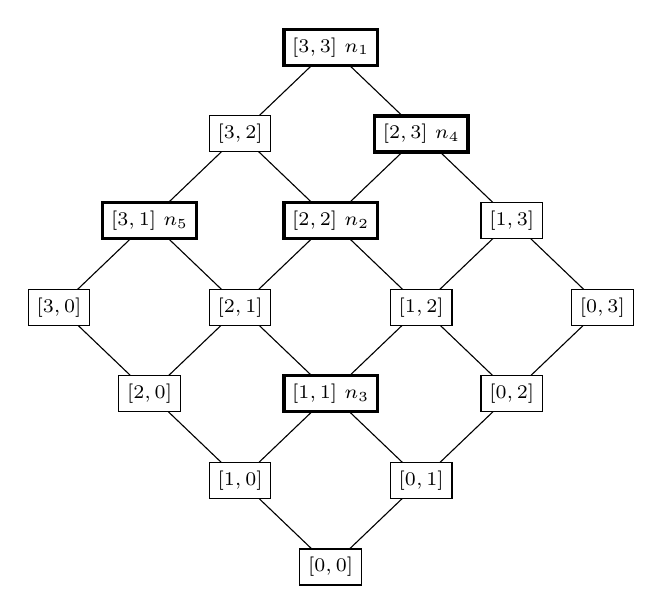
\begin{tikzpicture}[
      xscale=1.15, yscale=1.1,
      lnode/.style={
        rectangle, draw=black, thin,
        inner sep=3pt, font=\scriptsize, fill=white
      },
      enode/.style={
        rectangle, draw=black, very thick,
        inner sep=3pt, font=\scriptsize, fill=white
      },
      edge/.style={thin, black}
    ]
    
    % --- EDGES ---
    \draw[edge] (0,0) -- (-1,1);
    \draw[edge] (0,0) -- (1,1);
    \draw[edge] (-1,1) -- (-2,2);
    \draw[edge] (-1,1) -- (0,2);
    \draw[edge] (1,1)  -- (0,2);
    \draw[edge] (1,1)  -- (2,2);
    \draw[edge] (-2,2) -- (-3,3);
    \draw[edge] (-2,2) -- (-1,3);
    \draw[edge] (0,2)  -- (-1,3);
    \draw[edge] (0,2)  -- (1,3);
    \draw[edge] (2,2)  -- (1,3);
    \draw[edge] (2,2)  -- (3,3);
    \draw[edge] (-3,3) -- (-2,4);
    \draw[edge] (-1,3) -- (-2,4);
    \draw[edge] (-1,3) -- (0,4);
    \draw[edge] (1,3)  -- (0,4);
    \draw[edge] (1,3)  -- (2,4);
    \draw[edge] (3,3)  -- (2,4);
    \draw[edge] (-2,4) -- (-1,5);
    \draw[edge] (0,4)  -- (-1,5);
    \draw[edge] (0,4)  -- (1,5);
    \draw[edge] (2,4)  -- (1,5);
    \draw[edge] (-1,5) -- (0,6);
    \draw[edge] (1,5)  -- (0,6);
    
    % --- NODI REGOLARI ---
    \node[lnode] at (0,0)  {$[0,0]$};
    \node[lnode] at (-1,1) {$[1,0]$};
    \node[lnode] at (1,1)  {$[0,1]$};
    \node[lnode] at (-2,2) {$[2,0]$};
    \node[lnode] at (2,2)  {$[0,2]$};
    \node[lnode] at (-3,3) {$[3,0]$};
    \node[lnode] at (-1,3) {$[2,1]$};
    \node[lnode] at (1,3)  {$[1,2]$};
    \node[lnode] at (3,3)  {$[0,3]$};
    \node[lnode] at (2,4)  {$[1,3]$};
    \node[lnode] at (-1,5) {$[3,2]$};
    
    % --- NODI ESEMPIO (bordo spesso) ---
    \node[enode] at (0,2)  {$[1,1]\ n_3$};
    \node[enode] at (-2,4) {$[3,1]\ n_5$};
    \node[enode] at (0,4)  {$[2,2]\ n_2$};
    \node[enode] at (1,5)  {$[2,3]\ n_4$};
    \node[enode] at (0,6)  {$[3,3]\ n_1$};
    
    \end{tikzpicture}
    \caption{Reticolo $\mathcal{H} = \langle \Gamma,\, \succeq \rangle$ per $\mathcal{P} = \{S,\, C\}$, dove il primo componente di ogni classe indica il livello di $S$ e il secondo il livello di $C$, con i nodi relativi all'esempio ricorrente evidenziati con bordo spesso.}
    \label{fig:reticolo_nodi}
\end{figure}

Il reticolo consente di confrontare i profili dei nodi in modo diretto. Come si può notare subito, il nodo $n_1$, con classe $[3,\,3]$, domina tutti gli altri nodi dell'esempio. Scendendo nel reticolo, $n_4 = [2,\,3]$ domina $n_2 = [2,\,2]$ e $n_3 = [1,\,1]$: rispetto a $n_2$ offre lo stesso livello di sicurezza ma una capacità computazionale superiore, mentre domina completamente $n_3$ avendo entrambi i livelli superiori. Analogamente, $n_5 = [3,\,1]$ domina $n_3 = [1,\,1]$, avendo sicurezza massima a parità di capacità computazionale.

Però come già accennato, non tutte le coppie di nodi sono confrontabili, e i nodi $n_5 = [3,\,1]$ e $n_2 = [2,\,2]$ ne sono un esempio: $n_5$ è superiore per sicurezza ($3 > 2$) ma inferiore per computazione ($1 < 2$) rispetto a $n_2$, e dunque nessuno dei due domina l'altro. Lo stesso vale per la coppia $n_4 = [2,\,3]$ e $n_5 = [3,\,1]$: $n_5$ offre una sicurezza più alta, ma una capacità computazionale inferiore. In questi casi quindi, il reticolo non impone un ordine globale, e la scelta tra i due nodi dipenderà esclusivamente dai requisiti richiesti.

% ------------------------------------------------------------ %

\subsection{Compatibilità tra Requisiti delle Entità e Nodi}
\label{subsec:compatibilita_task_nodi}

Stabilita la classificazione dei nodi alla Sezione~\ref{subsec:classificazione_nodi} tramite le classi di proprietà $\alpha(n) \in \Gamma$, è ora possibile introdurre la controparte per i task e i dataset da essi richiesti. Come introdotto al capitolo precedente nella Sezione~\ref{sec:formalizzazione_base}, a ogni task $t \in \mathcal{T}$ è associato l'insieme $req(t) \subseteq \mathcal{D}$ dei dataset necessari alla sua esecuzione, e ogni task porta con sé un insieme di requisiti che esprimono le condizioni minime che il nodo di esecuzione deve soddisfare rispetto alle proprietà astratte in $\mathcal{P}$. Analogamente, ogni dataset $d \in \mathcal{D}$ dichiara requisiti di protezione propri, che vincolano qualsiasi nodo lo ospiti o lo elabori da remoto. Poiché entrambi i tipi di requisiti si esprimono nello stesso spazio $\Gamma = \mathcal{L}_{p_1} \times \ldots \times \mathcal{L}_{p_m}$ in cui i nodi sono classificati, la verifica di compatibilità si riduce a un confronto diretto tra livelli nel reticolo $\mathcal{H} = \langle \Gamma,\, \succeq \rangle$.

Definiamo ora quindi la controparte di $\alpha(n)$ per le classi di proprietà richieste dalle entità dei task e dei dataset.

\begin{definition}[Classe di proprietà richiesta da un'entità]
    \label{def:classe_richiesta}
    Dato un insieme di proprietà astratte $\mathcal{P} = \{p_1,\, \ldots,\, p_m\}$, la classe di proprietà richiesta di un'entità $x \in \mathcal{T} \cup \mathcal{D}$ è il vettore dato dalla funzione $\beta : \mathcal{T} \cup \mathcal{D} \rightarrow \Gamma$ tale che:
    \begin{equation}
        \beta(x) = \left[ \beta_p(x) \right]_{p \in \mathcal{P}}
    \end{equation}
    dove $\beta_p(x) \in \mathcal{L}_p$ è il livello minimo richiesto da $x$ per la proprietà $p$.
\end{definition}

La funzione $\beta$ è definita in modo uniforme su task e dataset, ma la sua semantica differisce a seconda del tipo di entità. Per un task $t \in \mathcal{T}$, il valore $\beta_p(t)$ esprime il livello minimo che il nodo di esecuzione deve possedere per la proprietà $p \in \mathcal{P}$ affinché il task possa essere eseguito correttamente. Per un dataset $d \in \mathcal{D}$, il valore $\beta_p(d)$ rappresenta invece il livello minimo di protezione che qualsiasi nodo deve garantire per ospitare o elaborare da remoto quel dataset, indipendentemente dalle dichiarazioni del task che lo richiede.

Riprendendo l'esempio ricorrente, supponiamo di voler sottomettere un task $t_1$ con classe di proprietà richiesta $\beta(t_1) = [1,\, 2]$, che necessita dei dataset $d_1$ e $d_2$, ossia $req(t_1) = \{d_1,\, d_2\}$. Il dataset $d_1$, che richiede determinate garanzie di sicurezza, ha $\beta(d_1) = [2,\, 1]$, mentre il dataset $d_2$, che richiede invece capacità computazionale elevata per essere elaborato correttamente, ha $\beta(d_2) = [1,\, 3]$.

Quindi, il task $t_1$ dichiara esplicitamente di necessitare di un nodo con $\beta_S(t_1) = 1$ per la sicurezza e $\beta_C(t_1) = 2$ per la computazione. Tuttavia, $d_1$ impone un requisito di sicurezza $\beta_S(d_1) = 2$ superiore a quanto dichiarato dal task stesso, mentre $d_2$ richiede un livello computazionale $\beta_C(d_2) = 3$ più elevato.

Dunque, il nodo di esecuzione dovrà soddisfare tutti questi vincoli contemporaneamente: non è sufficiente rispettare i soli requisiti del task né quelli di un singolo dataset, ma è necessario rispettarli tutti. Per catturare questo vincolo, si introduce la classe di proprietà effettiva richiesta da un task come il \emph{least upper bound} nel reticolo $\mathcal{H}$ tra la classe del task e quelle di tutti i dataset richiesti.

\begin{definition}[Classe di proprietà effettiva richiesta da un task]
    \label{def:classe_effettiva}
    Dato un task $t \in \mathcal{T}$ con $req(t) \subseteq \mathcal{D}$, la classe di proprietà effettiva $\beta^* : \mathcal{T} \rightarrow \Gamma$ è definita come il \emph{least upper bound} nel reticolo $\mathcal{H} = \langle \Gamma,\, \succeq \rangle$ tra la classe richiesta del task e quelle di tutti i dataset richiesti:
    \begin{equation}
        \beta^*(t) = \beta(t) \sqcup \left( \bigsqcup_{d \in req(t)} \beta(d) \right)
    \end{equation}
    Equivalentemente, poiché l'operatore $\sqcup$ è definito componente per componente come il massimo nei relativi insiemi totalmente ordinati $\mathcal{L}_p$, si ottiene:
    \begin{equation}
        \beta^*(t) = \left[ \max 
            \left( \beta_p(t),\, \max_{d \in req(t)} \beta_p(d) \right) 
        \right]_{p \in \mathcal{P}}
    \end{equation}
\end{definition}

Per costruzione quindi, $\beta^*(t) \succeq \beta(t)$ e $\beta^*(t) \succeq \beta(d)$ per ogni $d \in req(t)$: la classe di proprietà effettiva domina componente per componente tutti i singoli requisiti che la compongono. Nell'esempio, la classe effettiva di $t_1$ si ottiene calcolando il \emph{least upper bound} tra $\beta(t_1)$, $\beta(d_1)$ e $\beta(d_2)$:
\begin{equation}
    \beta^*(t_1)
    = \bigl[ \max(1,\,2,\,1),\;\max(2,\,1,\,3) \bigr]
    = [2,\,3]
\end{equation}
Come atteso, $\beta^*(t_1) = [2,\, 3]$ domina nel reticolo $\mathcal{H}$ sia $\beta(t_1) = [1,\, 2]$ sia $\beta(d_1) = [2,\, 1]$ sia $\beta(d_2) = [1,\, 3]$.

È ora possibile definire la prima politica concreta che formalizza la condizione di ammissibilità di un nodo rispetto ai requisiti effettivi di un task.

\begin{policy}[Politica di compatibilità delle proprietà $c_{prop}$]
    \label{pol:cprop}
    Dato un task $t \in \mathcal{T}$ e un nodo $n \in \mathcal{N}$, la politica $c_{prop} \in \mathcal{C_T} \cap \mathcal{C_D}$ è soddisfatta se e solo se la classe di proprietà del nodo domina la classe di proprietà effettiva del task nel reticolo $\mathcal{H} = \langle \Gamma,\, \succeq \rangle$:
    \begin{equation}
        n \models_t c_{prop}
        \iff
        \alpha(n) \succeq \beta^*(t)
        \iff
        \forall\, p \in \mathcal{P}:\; \alpha_p(n) \geq \beta^*_p(t)
    \end{equation}
\end{policy}

Grazie al Teorema~\ref{teo:soddisfacibilita_livelli}, la verifica di $\alpha_p(n) \geq \beta^*_p(t)$ per ogni $p \in \mathcal{P}$ si riduce a un confronto tra i valori interi delle classi, senza necessità di rivalutare le espressioni booleane sugli attributi dei nodi a ogni sottomissione di task.

Si osservi inoltre che la condizione $\alpha(n) \succeq \beta^*(t)$, per costruzione di $\beta^*(t)$ come \emph{least upper bound}, incorpora già i requisiti di protezione $\beta(d)$ di ogni $d \in req(t)$: un nodo che supera il filtro di $c_{prop}$ soddisfa automaticamente le condizioni minime richieste da ciascun dataset, risultando quindi candidato ammissibile per il loro eventuale trasferimento o accesso remoto. Ne consegue infatti che $c_{prop}$ appartiene sia all'insieme di politiche $\mathcal{C_T}$ che a $\mathcal{C_D}$. 

Questa proprietà sarà approfondita nel Teorema~\ref{teo:sussunzione_prop}, dopo aver introdotto la politica $c_{prop}^{\mathcal{D}} \in \mathcal{C_D}$ che esprime il vincolo di compatibilità delle proprietà a livello di singolo dataset: il teorema dimostrerà che la soddisfacibilità di $c_{prop}$ implica automaticamente anche quella di $c_{prop}^{\mathcal{D}}$ per ogni $d \in req(t)$. Applicando $c_{prop}$ all'esempio ricorrente con $\beta^*(t_1) = [2,\, 3]$, si confronta la classe di ciascun nodo della Tabella~\ref{tab:classi_nodi} componente per componente.

\begin{table}[ht]
    \centering
    \begin{tabular}{cc|cc|cc|c}
        \toprule
        \textbf{Nodo} & $\alpha(n)$ & $\alpha_S(n)$ & $\alpha_C(n)$ & $\alpha_S(n) \geq 2$ & $\alpha_C(n) \geq 3$ & Ammesso \\
        \midrule
        $n_1$ & $[3,\,3]$ & 3 & 3 & \checkmark & \checkmark & \checkmark \\
        $n_2$ & $[2,\,2]$ & 2 & 2 & \checkmark & \ding{55}  & \ding{55}  \\
        $n_3$ & $[1,\,1]$ & 1 & 1 & \ding{55}  & \ding{55}  & \ding{55}  \\
        $n_4$ & $[2,\,3]$ & 2 & 3 & \checkmark & \checkmark & \checkmark \\
        $n_5$ & $[3,\,1]$ & 3 & 1 & \checkmark & \ding{55}  & \ding{55}  \\
        \bottomrule
    \end{tabular}
    \caption{Applicazione di $c_{prop}$ sui nodi dell'esempio ricorrente dato il task $t_1$ con $\beta^*(t_1) = [2,\, 3]$.}
    \label{tab:cprop_t1}
\end{table}

Come si osserva dai risultati della Tabella~\ref{tab:cprop_t1}, l'insieme dei nodi ammissibili risulta essere $\mathcal{F}_{c_{prop}}(t_1) = \{n_1,\, n_4\}$. Tra questi, $n_4$ con classe $[2,\, 3]$ coincide esattamente con $\beta^*(t_1)$, senza alcun eccesso su nessuna proprietà, mentre $n_1$ con classe $[3,\, 3]$ offre un livello di sicurezza superiore al necessario. 

La scelta finale tra i due nodi sarà demandata all'indicatore dell'eccesso $\phi_{prop}$, introdotto nel seguito di questa sezione all'Indicatore~\ref{def:indicatore_eccesso}, che ottimizza la selezione verso il nodo ammissibile la cui classe è più vicina a $\beta^*(t)$ nel reticolo $\mathcal{H}$, minimizzando le risorse in eccesso rispetto a quanto strettamente necessario.

Si introduce ora la politica $c_{prop}^{\mathcal{D}} \in \mathcal{C_D}$, che esprime la condizione di compatibilità delle proprietà a livello di singolo dataset: il nodo candidato deve soddisfare i requisiti di protezione dichiarati dal dataset, indipendentemente dal task che lo richiede.

\begin{policy}[Politica di compatibilità delle proprietà dei dataset $c_{prop}^{\mathcal{D}}$]
    \label{pol:cprop_D}
    Dato un dataset $d \in \mathcal{D}$ e un nodo $n \in \mathcal{N}$, la politica $c_{prop}^{\mathcal{D}} \in \mathcal{C_D}$ è soddisfatta se e solo se la classe di proprietà del nodo domina la classe di proprietà richiesta dal dataset nel reticolo $\mathcal{H} = \langle \Gamma,\, \succeq \rangle$:
    \begin{equation}
        n \models_d c_{prop}^{\mathcal{D}}
        \iff
        \alpha(n) \succeq \beta(d)
        \iff
        \forall\, p \in \mathcal{P}:\; \alpha_p(n) \geq \beta_p(d)
    \end{equation}
\end{policy}

Ora, come anticipato, si dimostra formalmente che la soddisfacibilità di $c_{prop}$ di un task $t \in \mathcal{T}$ implica automaticamente la soddisfacibilità di $c_{prop}^{\mathcal{D}}$ per ogni dataset $d \in req(t)$ grazie alla costruzione di $\beta^*(t)$.

\begin{theorem}[Sussunzione di $c_{prop}^{\mathcal{D}}$ da parte di $c_{prop}$]
    \label{teo:sussunzione_prop}
    Per ogni task $t \in \mathcal{T}$ e ogni nodo $n \in \mathcal{N}$, se $n$ soddisfa $c_{prop}$ rispetto a $t$, allora soddisfa anche $c_{prop}^{\mathcal{D}}$ rispetto a ogni dataset richiesto da $t$:
    \begin{equation}
        n \models_t c_{prop}
        \implies
        \forall\, d \in req(t) :\; n \models_d c_{prop}^{\mathcal{D}}
        \qquad
        \forall\, t \in \mathcal{T},\, \forall\, n \in \mathcal{N}
    \end{equation}
    \begin{proof}
        Sia $n \models_t c_{prop}$, dunque $\alpha(n) \succeq \beta^*(t)$, il che significa $\alpha_p(n) \geq \beta^*_p(t)$ per ogni $p \in \mathcal{P}$. Dalla Definizione~\ref{def:classe_effettiva}, per ogni $d \in req(t)$ vale:
        \begin{equation}
            \beta^*_p(t)
            = \max\Bigl(\beta_p(t),\, \max_{d' \in req(t)} \beta_p(d')\Bigr)
            \geq \beta_p(d)
            \qquad
            \forall\, p \in \mathcal{P}
        \end{equation} 
        
        Quindi $\alpha_p(n) \geq \beta^*_p(t) \geq \beta_p(d)$ per ogni $d \in req(t)$ e ogni $p \in \mathcal{P}$, ovvero $\alpha(n) \succeq \beta(d)$, da cui $n \models_d c_{prop}^{\mathcal{D}}$ per ogni $d \in req(t)$.
    \end{proof}
\end{theorem}

È quindi dimostrato che $c_{prop}$ implica $c_{prop}^{\mathcal{D}}$ per tutti i dataset richiesti, giustificando formalmente l'appartenenza di $c_{prop}$ a $\mathcal{C_D}$. Di conseguenza, non è richiesta una verifica separata di $c_{prop}^{\mathcal{D}}$ quando $c_{prop}$ risulta già soddisfatta. Come si può notare dall'esempio ricorrente, i nodi ammissibili $\{n_1,\, n_4\}$ soddisfano entrambi $\alpha(n) \succeq [2,\, 3] = \beta^*(t_1)$, e per il Teorema~\ref{teo:sussunzione_prop}, soddisfano automaticamente $c_{prop}^{\mathcal{D}}$ sia per $d_1$, con $\beta(d_1) = [2,\, 1]$, sia per $d_2$, con $\beta(d_2) = [1,\, 3]$.

Dunque, la politica $c_{prop}$ opera come filtro, escludendo tutti i nodi per cui $\alpha(n) \not\succeq \beta^*(t)$, senza distinguere tra i nodi ammissibili rimasti. Tuttavia, come anticipato nell'esempio, tra i nodi che superano il filtro possono esistere differenze significative: un nodo con $\alpha(n) = \beta^*(t)$ utilizza esattamente le risorse richieste, mentre un nodo con $\alpha(n) \succ \beta^*(t)$ offre capacità in eccesso rispetto ai requisiti. Perciò, a parità di ammissibilità, è preferibile evitare sprechi assegnando il task al nodo la cui classe di proprietà è più vicina a $\beta^*(t)$ nel reticolo $\mathcal{H}$: si vuole, in altri termini, il nodo che soddisfa i requisiti con il minore eccesso possibile.

Un nodo $n \models_t c_{prop}$ la cui classe di proprietà coincide esattamente con la classe effettiva richiesta dal task, ossia $\alpha(n) = \beta^*(t)$, rappresenta quindi il caso ottimo, definendo $n$ come nodo ideale per $t$. Un nodo di questo tipo, quando esiste, è la scelta migliore rispetto al principio del minimo privilegio~\cite{least-privilege}, dato che consente l'esecuzione del task senza sprecare risorse per nessuna proprietà. Tale principio, fondamentale per la sicurezza dei sistemi informatici, impone infatti che un'entità operi strettamente con il livello di autorizzazione e di risorse necessario al suo funzionamento, al fine di ridurre la superficie di attacco e mantenere il corretto isolamento.

Va osservato, tuttavia, che un nodo ideale potrebbe non essere sempre presente o disponibile nel cluster nel momento del bisogno. In questo caso, nessun nodo raggiungerebbe il minimo teorico ottimo e la selezione dovrebbe orientarsi verso il nodo ammissibile ottimale più vicino a $\beta^*(t)$. Questo criterio di ottimalità sarà catturato dall'indicatore dell'eccesso di proprietà $\phi_{prop}$, che quantifica lo scarto componente per componente tra la classe del nodo e la classe effettiva richiesta.

Ora, considerando lo scarto tra le classi di proprietà come la distanza di Manhattan nel reticolo $\mathcal{H}$ tra $\alpha(n)$ e $\beta^*(t)$, ossia: 
\begin{equation}
    \sum_{p \in \mathcal{P}}\left(\alpha_p(n) - \beta^*_p(t)\right)
\end{equation}
si avrà, per costruzione di $c_{prop}$, un valore sempre non negativo per ogni nodo ammissibile $n \models_t c_{prop}$, con valore nullo se e solo se $n$ è un nodo ideale per $t$, ovvero $\alpha(n) = \beta^*(t)$. 

Tuttavia, questa misura grezza tratterebbe tutte le proprietà in modo uniforme e non permetterebbe la distinzione tra proprietà con livelli differenti: uno scarto di $2$ livelli su una proprietà con $3$ livelli totali è ben più significativo dello stesso scarto su una proprietà con $10$ livelli. Sarebbe quindi opportuno normalizzare il contributo di ciascuna proprietà rispetto al massimo scarto possibile, riportandolo in un intervallo standard $[0,\, 1]$. 

Inoltre, poiché non tutte le proprietà hanno necessariamente la stessa rilevanza nell'economia globale del sistema, si introduce un vettore di pesi:
\begin{equation}
    \overline{w}_{\mathcal{P}} = [w_p]_{p \in \mathcal{P}} \in \mathbb{R}^{|\mathcal{P}|}
\end{equation}
che associa a ciascuna proprietà $p \in \mathcal{P}$ un peso $w_p > 0$. Questo perché, in uno scenario reale, un eccesso sul livello di sicurezza potrebbe avere conseguenze più rilevanti, in termini di risorse dedicate e garanzie offerte, rispetto a un eccesso sulla capacità computazionale.

Con questi presupposti, dato un vettore di pesi $\overline{w}_{\mathcal{P}}$ per un insieme di proprietà $\mathcal{P}$, è ora possibile definire l'eccesso di proprietà normalizzato e pesato tra la classe di un nodo $n \in \mathcal{N}$ e la classe effettiva richiesta da un task $t \in \mathcal{T}$ come:
\begin{equation}
    \label{eq:eccesso_norm}
    \Delta(n,\, t) = \sum_{\substack{p \in \mathcal{P} \\ \beta^*_p(t) < \max \mathcal{L}_p}} 
    w_p \frac{\alpha_p(n) - \beta^*_p(t)}{\max \mathcal{L}_p - \beta^*_p(t)}
\end{equation}
Per convenzione, le proprietà per cui $\beta^*_p(t) = \max \mathcal{L}_p$ non sono incluse nella sommatoria, poiché in tal caso ogni nodo ammissibile avrebbe necessariamente $\alpha_p(n) = \max \mathcal{L}_p$, risultando non discriminante e con contributo nullo all'eccesso. Inoltre, per costruzione di $c_{prop}$, $\Delta(n,\, t) \geq 0$ per ogni nodo $n \models_t c_{prop}$, con $\Delta(n,\, t) = 0$ se e solo se $n$ è un nodo ideale per $t$, ovvero $\alpha(n) = \beta^*(t)$.

Dato che ciascun rapporto normalizzato:
\begin{equation}
    \frac{\alpha_p(n) - \beta^*_p(t)}{\max \mathcal{L}_p - \beta^*_p(t)}
\end{equation}
assume valori nell'intervallo $[0,\,1]$ per ogni nodo ammissibile $n \models_t c_{prop}$, la somma pesata $\Delta(n,\, t)$ risulta limitata superiormente dalla somma dei pesi delle proprietà che contribuiscono alla sommatoria. Questo limite viene indicato con:
\begin{equation}
    \Delta_{max}(t) = \sum_{\substack{p \in \mathcal{P} \\ \beta^*_p(t) < \max \mathcal{L}_p}} w_p
\end{equation}
Il valore $\Delta_{max}(t)$ dipende esclusivamente dal task $t$ e dal vettore di pesi $\overline{w}_{\mathcal{P}}$, non dal nodo candidato, ed è quindi calcolabile una sola volta per ciascun task al momento della sua sottomissione. Per costruzione, vale dunque $0 \leq \Delta(n,\,t) \leq \Delta_{max}(t)$ per ogni nodo ammissibile $n \models_t c_{prop}$.

A partire dall'eccesso così definito e dal suo limite superiore, l'indicatore $\phi_{prop}$ traduce lo scarto in un punteggio normalizzato direttamente integrabile nella funzione di ottimizzazione.

\begin{optimizer}[Indicatore dell'eccesso di proprietà $\phi_{prop}$]
    \label{def:indicatore_eccesso}
    Sia $\mathcal{C}$ l'insieme delle politiche del sistema. Dato un task $t \in \mathcal{T}$, un nodo candidato $n \in \mathcal{N}$ tale per cui $n \in \mathcal{F_C}(t)$ e un vettore di pesi $\overline{w}_{\mathcal{P}}$ per un insieme di proprietà $\mathcal{P}$, l'indicatore dell'eccesso di proprietà $\phi_{prop} \in \Phi$ è definito
    come:
    \begin{equation}
        \phi_{prop}(n,\, t) = 
        \begin{cases} 
            1 - \dfrac{\Delta(n,\, t)}{\Delta_{max}(t)} & \text{se } \Delta_{max}(t) > 0 \\[2ex]
            1 & \text{se } \Delta_{max}(t) = 0
       \end{cases}
    \end{equation}
    Per convenzione, nel caso in cui nessuna proprietà contribuisca alla sommatoria dell'eccesso avendo $\Delta_{max}(t) = 0$, si ha $\phi_{prop}(n,\, t) = 1$.
\end{optimizer}

L'indicatore $\phi_{prop}$ raggiunge il valore massimo $1$ se e solo se $n$ è un nodo ideale per $t$, cioè quando $\Delta(n,\, t) = 0$, e raggiunge il valore minimo $0$ quando $\Delta(n,\, t) = \Delta_{max}(t)$, ovvero quando il nodo satura al proprio massimo livello $\max \mathcal{L}_p$ ogni proprietà $p$ che contribuisce alla sommatoria dell'eccesso. Tra questi due estremi, $\phi_{prop}$ decresce linearmente al crescere dell'eccesso di proprietà: a incrementi uguali di $\Delta(n,\, t)$ corrispondono decrementi uguali nel punteggio, garantendo una penalizzazione proporzionale. Questa decrescita garantisce che nodi con un eccesso $\Delta(n,\, t)$ maggiore ricevano sempre un punteggio inferiore rispetto a nodi con eccesso minore, producendo un ordinamento dei candidati coerente con il principio del minimo privilegio. 

Dall'esempio ricorrente, con $\beta^*(t_1) = [2,\, 3]$ e $\mathcal{L}_S = \mathcal{L}_C = \{0,\, 1,\, 2,\, 3\}$, la proprietà $C$ risulta esclusa dalla sommatoria dell'eccesso dato che $\beta^*_C(t_1) = \max \mathcal{L}_C = 3$: nessun nodo ammissibile può eccedere per $C$. L'unica proprietà rilevante rimane quindi $S$. Adottando $w_S = 1$, si ha $\Delta_{max}(t_1) = w_S = 1$, e i due nodi ammissibili producono:
\begin{align}
    &\Delta(n_4,\, t_1) = \frac{2 - 2}{3 - 2} = 0
    \implies \phi_{prop}(n_4,\, t_1) = 1 - \frac{0}{1} = 1 \\
    &\Delta(n_1,\, t_1) = \frac{3 - 2}{3 - 2} = 1
    \implies \phi_{prop}(n_1,\, t_1) = 1 - \frac{1}{1} = 0
\end{align}
Come previsto, il nodo $n_4$, la cui classe $[2,\, 3]$ coincide esattamente con $\beta^*(t_1)$, risulta essere il nodo ideale per $t_1$ ottenendo il punteggio massimo. Il nodo $n_1$ invece, con classe $[3,\, 3]$, satura l'eccesso dell'unica proprietà rilevante $S$ al proprio massimo livello, ottenendo il punteggio minimo tra i candidati ammissibili. In assenza di altri indicatori nella funzione di ottimizzazione, il sistema selezionerebbe $n_4$ come nodo ottimale, confermando che il nodo ideale, quando presente nel cluster, è la scelta ottima.

% ------------------------------------------------------------ %

\section{Localizzazione Geografica dei Nodi e delle Entità}
\label{sec:localizzazione_geografica}

Un secondo aspetto riguarda la collocazione fisica dei nodi e i vincoli di sovranità geografica che ne derivano. Si definisce prima un modello di raggruppamento gerarchico delle località del cluster, per poi introdurre la politica $c_{geo}$ che vincola l'assegnazione dei task e il trasferimento dei dataset ai soli nodi collocati in aree geografiche autorizzate.

% ------------------------------------------------------------ %

\subsection{Raggruppamento Geografico dei Nodi}
\label{subsec:raggruppamento_geografico}

La classificazione per proprietà astratte introdotta precedentemente alla Sezione~\ref{subsec:classificazione_nodi} classifica i nodi del cluster rispetto a dimensioni derivate dalle loro caratteristiche tecniche, senza però tenere conto della loro collocazione fisica. Tuttavia, in molti contesti applicativi la posizione geografica di un nodo è un elemento vincolante tanto quanto le sue proprietà tecniche. Il concetto di \emph{data sovereignty}, inteso come il controllo esercitabile su un dato in base alle leggi e alla giurisdizione del territorio in cui esso viene trattato o archiviato~\cite{data-sovereignty-review}, si traduce concretamente in normative sulla residenza dei dati, come il Regolamento Generale sulla Protezione dei Dati (GDPR) in ambito europeo, o accordi internazionali che limitano il trattamento di determinate informazioni a specifici territori; ad oggi, provvedimenti di questo tipo sono adottati da un numero sempre maggiore di giurisdizioni a livello globale~\cite{oecd-data-localisation}. Questi vincoli potrebbero imporre che certi task vengano eseguiti soltanto su nodi situati in aree geografiche espressamente autorizzate. Analogamente, un dataset soggetto a requisiti di sovranità potrebbe non essere trasferito né elaborato su nodi che si trovino al di fuori dell'area di competenza dichiarata.

Per catturare questi vincoli, coerentemente con soluzioni già note per il controllo della collocazione fisica dei dati su infrastrutture cloud~\cite{geolocation-aware-data-placement}, si introduce un modello di raggruppamento geografico dei nodi complementare alla classificazione per proprietà. L'idea fondamentale è separare la posizione concreta di ciascun nodo, espressa come una singola località, dalla nozione più astratta di gruppo geografico, ovvero un insieme di località che condividono uno spazio comune dal punto di vista normativo o organizzativo. I vincoli di un task o di un dataset si esprimeranno in termini di gruppi geografici, mentre i nodi dichiareranno la propria località individuale. La verifica di compatibilità si riduce quindi a stabilire se la località di un nodo appartenga all'insieme di località che compone il gruppo richiesto.

Per iniziare, si introduce l'insieme di tutte le località geografiche possibili dei nodi del cluster con $\Omega$. Inoltre, ogni nodo $n \in \mathcal{N}$ sarà associato a una singola località tramite la funzione:
\begin{equation}
    loc: \mathcal{N} \rightarrow \Omega
\end{equation}
dove $loc(n)$ indica la località geografica del nodo $n$, ovvero la sua regione di appartenenza.
 
Considerando il seguente insieme universale delle località: 
\begin{equation}
    \Omega = \left\{ 
    \begin{aligned}
        &\mathtt{eu\text{-}north},\, \mathtt{eu\text{-}south},\, \mathtt{eu\text{-}east},\, \mathtt{eu\text{-}west},
        \\
        &\mathtt{us\text{-}north},\, \mathtt{us\text{-}south},\, \mathtt{us\text{-}east},\, \mathtt{us\text{-}west},
        \\
        &\mathtt{apac\text{-}east}
    \end{aligned}
    \right\}
\end{equation} 

si estende la descrizione dei nodi di esempio della Tabella~\ref{tab:attributi_nodi} con l'attributo $loc$, assegnando a ciascun nodo una località geografica come riportato nella Tabella~\ref{tab:localita_nodi}.

\begin{table}[ht]
    \centering
    \begin{tabular}{cc}
        \toprule
        \textbf{Nodo} & $loc(n)$ \\
        \midrule
        $n_1$ & \texttt{eu-west}  \\
        $n_2$ & \texttt{eu-north} \\
        $n_3$ & \texttt{us-west} \\
        $n_4$ & \texttt{eu-south} \\
        $n_5$ & \texttt{apac-east} \\
        \bottomrule
    \end{tabular}
    \caption{Località geografiche dei nodi nell'esempio ricorrente.}
    \label{tab:localita_nodi}
\end{table}

I gruppi geografici invece sono insiemi di località che condividono una normativa o organizzazione comune. Un nodo apparterrà implicitamente a tutti i gruppi che contengono la sua località: non c'è una relazione di appartenenza esplicita tra nodi e gruppi, ma deriva direttamente dall'inclusione di $loc(n)$ nell'insieme di località che definirà ciascun gruppo.

\begin{definition}[Gruppi geografici]
    \label{def:gruppi_geografici}
    Sia $\Omega$ l'insieme delle località considerate. Un insieme di gruppi geografici è una famiglia $\mathcal{G} \subseteq 2^{\Omega}$ i cui elementi $g \in \mathcal{G}$ rappresentano sottoinsiemi di località geograficamente o normativamente affini. Si assume che $\Omega \in \mathcal{G}$, ossia che il gruppo universale sia sempre incluso nella famiglia e rappresenti l'assenza di qualsiasi vincolo geografico specifico. 
\end{definition}

La famiglia $\mathcal{G}$ non è necessariamente una partizione di $\Omega$: i gruppi possono sovrapporsi e generare relazioni gerarchiche. Sono quindi ammessi gruppi composti $g \in \mathcal{G}$ tali che:
\begin{equation}
    g = \left( \bigcup_{i=1}^{m} g_i \right) \cup G
\end{equation}
dove $g_i \in \mathcal{G}$ per ogni $i \in \{1,\dots,m\}$ e $G \subseteq \Omega$ indica l'eventuale parte del gruppo non inclusa in ulteriori sottogruppi di $\mathcal{G}$. Questi gruppi composti permettono di modellare aggregazioni geografiche o normative non banali, ottenute dalla combinazione di aree già definite all'interno della struttura gerarchica di $\mathcal{G}$. 

Riprendendo l'esempio ricorrente, i gruppi geografici definiti sono riportati nella Tabella~\ref{tab:gruppi_geografici}, dove $\mathtt{OECD}$ è un esempio di gruppo composto. Si ottiene così la famiglia $\mathcal{G} = \left\{ \mathtt{EU},\, \mathtt{US},\, \mathtt{OECD},\, \Omega \right\}$.
 
\begin{table}[ht]
    \centering
    \begin{tabular}{cl}
        \toprule
        \textbf{Gruppo} & \textbf{Località} \\
        \midrule
        $\mathtt{EU}$ & 
        $\left\{ \mathtt{eu\text{-}north},\, \mathtt{eu\text{-}south},\, \mathtt{eu\text{-}east},\, \mathtt{eu\text{-}west} \right\}$ 
        \\
        $\mathtt{US}$ & 
        $\left\{ \mathtt{us\text{-}north},\, \mathtt{us\text{-}south},\, \mathtt{us\text{-}east},\, \mathtt{us\text{-}west} \right\}$ 
        \\
        $\mathtt{OECD}$ & 
        $\mathtt{EU} \cup \mathtt{US}$ 
        \\
        \bottomrule
    \end{tabular}
    \caption{Gruppi geografici $\mathcal{G}$ nell'esempio ricorrente, dove per semplicità è omesso il gruppo $\Omega$.}
    \label{tab:gruppi_geografici}
\end{table}

La Figura~\ref{fig:gruppi_geografici} illustra graficamente la struttura di annidamento dei gruppi e la relativa distribuzione delle località.

\begin{figure}[ht]
    \centering
    \begin{tikzpicture}[
        every node/.style={font=\small},
        % Stile per le etichette dei gruppi (EU, US, OECD, Omega)
        group label/.style={font=\large\bfseries, text depth=0pt},
        % Stile per i pallini delle località
        loc/.style={circle, fill=black!80, draw=white, thick, inner sep=1.5pt},
        % Stili per le forme degli insiemi
        omega box/.style={thick, rounded corners=8pt, fill=black!2, draw=black!70},
        oecd box/.style={thick, rounded corners=12pt, fill=diogreen!60, draw=diogreenborder},
        eu ellipse/.style={thick, fill=dioblue, draw=dioblueborder},
        us ellipse/.style={thick, fill=diored!70, draw=dioredborder},
        % Stile per il testo delle località
        loc lab/.style={font=\ttfamily\footnotesize, text=black}
    ]

    % --- Insieme Universale Omega (ridotto per stare nei margini) ---
    \draw[omega box] (-7.2,-3.8) rectangle (7.2,3.8);
    \node[group label, text=black!80] at (6.6, 3.2) {$\Omega$};

    % --- OECD (ridotto e adattato) ---
    \draw[oecd box] (-5.8,-2.8) rectangle (5.8,2.8);
    \node[group label, text=diogreenborder!80!black] at (-4.8, 2.2) {$\mathtt{OECD}$};

    % --- EU ed US (avvicinati al centro) ---
    \draw[eu ellipse] (-2.8,0) ellipse (2.25cm and 2.25cm);
    \node[group label, text=dioblueborder!80!black] at (-2.8, 1.5) {$\mathtt{EU}$};

    \draw[us ellipse] (2.8,0) ellipse (2.25cm and 2.25cm);
    \node[group label, text=dioredborder] at (2.8, 1.5) {$\mathtt{US}$};
    
    % --- LOCALITÀ EU ---
    % Etichette disposte a croce verso l'esterno
    \node[loc, label={[loc lab]below:eu-west}]  at (-4.0,  0.0) {};
    \node[loc, label={[loc lab]below:eu-east}]  at (-1.6,  0.0) {};
    \node[loc, label={[loc lab]below:eu-north}] at (-2.8,  0.8) {};
    \node[loc, label={[loc lab]below:eu-south}] at (-2.8, -0.8) {};

    % --- LOCALITÀ US ---
    \node[loc, label={[loc lab]below:us-west}]  at (1.6,  0.0) {};
    \node[loc, label={[loc lab]below:us-east}]  at (4.0,  0.0) {};
    \node[loc, label={[loc lab]below:us-north}] at (2.8,  0.8) {};
    \node[loc, label={[loc lab]below:us-south}] at (2.8, -0.8) {};

    % --- LOCALITÀ APAC ---
    % Riposizionata in basso a destra, con testo verso l'alto per non toccare il bordo
    \node[loc, label={[loc lab]left:apac-east}] at (6.5, -3.2) {};

    \end{tikzpicture}
    \caption{Struttura dei gruppi geografici $\mathcal{G}$ e distribuzione di tutte le località $\Omega$ nell'esempio ricorrente.}
    \label{fig:gruppi_geografici}
\end{figure}

Volendo verificare l'appartenenza dei nodi dell'esempio ricorrente relativi alla Tabella~\ref{tab:localita_nodi} ai gruppi geografici definiti in $\mathcal{G}$, si osserva che i nodi $n_1$, $n_2$ e $n_4$, tutti situati in località europee, appartengono simultaneamente a $\mathtt{EU}$, $\mathtt{OECD}$ e $\Omega$; il nodo $n_3$, situato negli Stati Uniti, appartiene a $\mathtt{US}$, $\mathtt{OECD}$ e $\Omega$; mentre il nodo $n_5$, la cui località non rientra in nessun gruppo definito al di fuori di quello universale, appartiene semplicemente a $\Omega$.

% ------------------------------------------------------------ %

\subsection{Co-locazione Geografica delle Entità nei Nodi}
\label{subsec:politica_geo}

Il raggruppamento geografico introdotto nella Sezione~\ref{subsec:raggruppamento_geografico} a questo punto offre gli strumenti necessari per esprimere vincoli di residenza geografica su task e dataset. In questa sezione si definirà la politica $c_{geo}$, che restringe l'insieme dei nodi candidati a quelli la cui località soddisfa simultaneamente i requisiti geografici dichiarati da un task $t \in \mathcal{T}$ e da tutti i suoi dataset richiesti $req(t) \subseteq \mathcal{D}$. Un approccio analogo, che tratta i vincoli normativi sulla collocazione dei dati come vincoli formali nel posizionamento dei processi su infrastrutture cloud distribuite geograficamente, è adottato in~\cite{privacy-regulation-aware-process-mapping}.

La struttura di questa politica ricalcherà quella già adottata precedentemente con la politica $c_{prop}$: a ciascuna entità è associato un requisito espresso nei termini del modello di raggruppamento geografico illustrato alla Sezione~\ref{subsec:raggruppamento_geografico}, da questi requisiti si deriva un raggruppamento effettivo univoco per il task che include anche i requisiti dei dataset, infine la politica filtra i nodi controllando che il raggruppamento effettivo ottenuto contenga la località geografica del nodo che si sta considerando.

\begin{definition}[Gruppo geografico richiesto da un'entità]
    \label{def:requisito_geografico}
    Dato un insieme di gruppi geografici $\mathcal{G}$, il gruppo geografico richiesto di un'entità $x \in \mathcal{T} \cup \mathcal{D}$ è dato da:
    \begin{equation}
        geo : \mathcal{T} \cup \mathcal{D} \rightarrow \mathcal{G}
    \end{equation}
    dove $geo(x)$ è il gruppo geografico al quale deve appartenere la località del nodo che esegue o elabora $x$. In particolare, un'entità senza vincoli di localizzazione viene indicata con $geo(x) = \Omega$, ovvero il gruppo universale. 
\end{definition}

Per un task $t \in \mathcal{T}$, $geo(t)$ esprime quindi il vincolo geografico richiesto dall'utente per l'esecuzione, ad esempio per rispettare normative di compliance o politiche aziendali. Per un dataset $d \in \mathcal{D}$ invece, $geo(d)$ rappresenta il vincolo di residenza dichiarato dal dataset stesso: qualsiasi nodo che lo ospiti dovrà trovarsi in una località appartenente a $geo(d)$, indipendentemente dal task che lo richiede.

Riprendendo l'esempio ricorrente con $req(t_1) = \left\{ d_1,\, d_2 \right\}$, si assegnano i requisiti geografici $geo(t_1) = \mathtt{EU}$, $geo(d_1) = \mathtt{OECD}$ e $geo(d_2) = \Omega$: il task $t_1$ richiede di essere eseguito su un nodo collocato in area europea, il dataset $d_1$ richiede un nodo collocato in un paese \texttt{OECD}, mentre il dataset $d_2$ non impone alcun vincolo geografico. Si osservi che, presi singolarmente, i tre requisiti non sono in conflitto tra loro: ogni località in $\mathtt{EU}$ appartiene anche a $\mathtt{OECD}$ e a $\Omega$, dunque un nodo con $loc(n) \in \mathtt{EU}$ soddisferebbe contemporaneamente tutti e tre i vincoli. 

Per stabilire questo formalmente senza confrontare i requisiti uno a uno, si definisce un unico raggruppamento effettivo che li includa tutti.

\begin{definition}[Gruppo geografico effettivo richiesto da un task]
    \label{def:localita_effettiva}
    Dato un task $t \in \mathcal{T}$ con $req(t) \subseteq \mathcal{D}$, si definisce l'insieme delle località effettivamente ammissibili per $t$ con $geo^* : \mathcal{T} \rightarrow 2^\Omega$, ovvero l'intersezione tra le località del gruppo geografico richiesto dal task e quelle di tutti i dataset richiesti:
    \begin{equation}
        geo^*(t) = geo(t) \cap \left( \bigcap_{d \in req(t)} geo(d) \right)
    \end{equation}
\end{definition}

L'insieme $geo^*(t)$ raccoglie ora tutte le località che soddisfano simultaneamente il vincolo del task e quelli di tutti i dataset richiesti. Si noti che, essendo $geo(x) \subseteq \Omega$ per ogni $x \in \mathcal{T} \cup \mathcal{D}$, anche $geo^*(t) \subseteq \Omega$, in particolare $geo^*(t)$ potrebbe risultare vuoto qualora i gruppi coinvolti siano in conflitto tra loro non avendo alcuna intersezione comune. 

Nell'esempio, la località effettiva di $t_1$ si ottiene calcolando l'intersezione tra $geo(t_1)$, $geo(d_1)$ e $geo(d_2)$, risultando:
\begin{equation}
    geo^*(t_1) = \mathtt{EU} \cap \mathtt{OECD} \cap \Omega = \mathtt{EU}
\end{equation}
poiché $\mathtt{EU} \subseteq \mathtt{OECD} \subseteq \Omega$, ottenendo come ci si aspettava dall'osservazione precedente il requisito più stringente tra i tre.

Da queste premesse, possiamo definire la politica di co-locazione geografica $c_{geo}$.

\begin{policy}[Politica di co-locazione geografica $c_{geo}$]
\label{pol:c_geo}
    Dato un task $t \in \mathcal{T}$ e un nodo $n \in \mathcal{N}$, la politica $c_{geo} \in \mathcal{C_T} \cap \mathcal{C_D}$ è soddisfatta se e solo se la località del nodo appartiene al raggruppamento geografico effettivo del task:
    \begin{equation}
        n \models_t c_{geo}
        \iff
        loc(n) \in geo^*(t)
    \end{equation}
\end{policy}

Nel caso in cui dovesse risultare $geo^*(t) = \emptyset$, nessun nodo per costruzione potrebbe soddisfare $c_{geo}$, e dunque il task non potrebbe essere assegnato a nessun nodo avendo $\mathcal{F}_{c_{geo}}(t) = \emptyset$. Applicando $c_{geo}$ all'esempio ricorrente con: 
\begin{equation}
    geo^*(t_1) = \mathtt{EU} = \{\mathtt{eu\text{-}north},\, \mathtt{eu\text{-}south},\, \mathtt{eu\text{-}east},\, \mathtt{eu\text{-}west}\}
\end{equation}
si verifica $loc(n) \in geo^*(t_1)$ per ciascun nodo della Tabella~\ref{tab:localita_nodi}. I nodi $n_1$, $n_2$ e $n_4$, con:
\begin{equation}
    loc(n) \in \{\mathtt{eu\text{-}west},\, \mathtt{eu\text{-}north},\, \mathtt{eu\text{-}south}\}  \subseteq geo^*(t_1) 
    \qquad
    n \in \left\{ n_1,\, n_2,\, n_4 \right\}
\end{equation}
soddisfano $c_{geo}$, mentre $n_3$ con $loc(n_3) = \mathtt{us\text{-}west} \notin \mathtt{EU}$, e $n_5$ con $loc(n_5) = \mathtt{apac\text{-}east} \notin \mathtt{EU}$, non lo soddisfano. L'insieme dei nodi ammissibili rispetto a $c_{geo}$ risulta essere quindi $\mathcal{F}_{c_{geo}}(t_1) = \left\{ n_1,\, n_2,\, n_4 \right\}$.
 
Si consideri ora la variante in cui $req(t_1) = \left\{ d_1,\, d_3 \right\}$ con $geo(d_3) = \mathtt{US}$. Il raggruppamento effettivo diventerebbe:
\begin{equation}
    geo^*(t_1) = \mathtt{EU} \cap \mathtt{OECD} \cap \mathtt{US} = \emptyset
\end{equation}
poiché $\mathtt{EU} \cap \mathtt{US} = \emptyset$, nessuna località appartiene contemporaneamente all'area europea e a quella statunitense. Come già accennato, $geo^*(t_1) = \emptyset$ implica che nessun nodo del cluster, indipendentemente dalle sue proprietà o dalla sua disponibilità, possa soddisfare $c_{geo}$, e dunque il task $t_1$ non sarebbe assegnato a nessun nodo. Questo è un classico caso di conflitto tra i requisiti di $t_1$ e $d_3$, rilevabile immediatamente al momento della sottomissione del task.

Si osservi inoltre che, analogamente a quanto mostrato per $c_{prop}$ alla Sezione~\ref{subsec:compatibilita_task_nodi}, anche $c_{geo}$ appartiene sia all'insieme di politiche $\mathcal{C_T}$ sia a $\mathcal{C_D}$, dato che la struttura di $geo^*$ rappresenta l'intersezione tra il gruppo geografico richiesto dal task e quelli associati a tutti i dataset richiesti. Questa proprietà sarà dimostrata formalmente nel Teorema~\ref{teo:sussunzione_geo}.

Si introduce ora la politica $c_{geo}^{\mathcal{D}} \in \mathcal{C_D}$ che considera esclusivamente i vincoli di co-locazione geografica a livello di singolo dataset.

\begin{policy}[Politica di co-locazione geografica dei dataset $c_{geo}^{\mathcal{D}}$]
    \label{pol:c_geo_dataset}
    Dato un dataset $d \in \mathcal{D}$ e un nodo $n \in \mathcal{N}$, la politica $c_{geo}^{\mathcal{D}} \in \mathcal{C_D}$ è soddisfatta se e solo se la località del nodo appartiene al gruppo geografico richiesto dal dataset:
    \begin{equation}
        n \models_d c_{geo}^{\mathcal{D}}
        \iff
        loc(n) \in geo(d)
    \end{equation}
\end{policy}

Anche in questo caso, dato un task $t \in \mathcal{T}$, la politica $c_{geo}^{\mathcal{D}}$ risulta automaticamente soddisfatta per ogni dataset $d \in req(t)$ se viene soddisfatta a priori $c_{geo}$, questo grazie alla struttura di $geo^*$.

\begin{theorem}[Sussunzione di $c_{geo}^{\mathcal{D}}$ da parte di $c_{geo}$]
\label{teo:sussunzione_geo}
    Per ogni task $t \in \mathcal{T}$ e nodo $n \in \mathcal{N}$, se $n$ soddisfa $c_{geo}$ rispetto a $t$, allora soddisfa anche $c_{geo}^{\mathcal{D}}$ rispetto a ogni dataset richiesto da $t$:
    \begin{equation}
        n \models_t c_{geo}
        \implies
        \forall\, d \in req(t) :\; n \models_d c_{geo}^{\mathcal{D}}
        \qquad
        \forall\, t \in \mathcal{T},\, \forall\, n \in \mathcal{N}
    \end{equation}
    \begin{proof}
        Sia $n \models_t c_{geo}$, il che implica $loc(n) \in geo^*(t)$. Dalla Definizione~\ref{def:localita_effettiva} per ogni $d \in req(t)$ si osserva che:
        \begin{equation}
            geo^*(t) = geo(t) \cap \left( \bigcap_{d' \in req(t)} geo(d') \right) \subseteq geo(d)
        \end{equation}
        essendo $geo^*(t)$ un'intersezione che include $geo(d)$ per ogni $d \in req(t)$ come operando. 
        
        Quindi $loc(n) \in geo^*(t)$ implica $loc(n) \in geo(d)$ per ogni $d \in req(t)$, da cui $n \models_d c_{geo}^{\mathcal{D}}$ per ogni $d \in req(t)$.
    \end{proof}
\end{theorem}

Questo risultato giustifica formalmente l'appartenenza di $c_{geo}$ anche alla famiglia di politiche $\mathcal{C_D}$, in quanto ingloba implicitamente il vincolo $c_{geo}^{\mathcal{D}}$ per ciascun dataset richiesto, evitando di conseguenza la verifica caso per caso di $c_{geo}^{\mathcal{D}}$.

Per finire, rifacendosi all'esempio, i nodi ammissibili per il task $t_1$ risultano $\left\{ n_1,\, n_2,\, n_4 \right\}$ rispetto a $c_{geo}$, e per il Teorema~\ref{teo:sussunzione_geo}, come dimostrato e facilmente verificabile, soddisfano automaticamente anche $c_{geo}^{\mathcal{D}}$ sia per $d_1$, con $geo(d_1) = \mathtt{OECD} \supseteq \mathtt{EU}$, sia per $d_2$, con $geo(d_2) = \Omega \supseteq \mathtt{EU}$.

% ------------------------------------------------------------ %
 
\section{Trasferimento e Località dei Dataset}
\label{sec:trasferimento_localita_dataset}

Il terzo aspetto riguarda la gestione dei dataset rispetto alla loro possibilità di essere trasferiti tra nodi. Si distingue innanzitutto la categoria dei dataset statici, per i quali il trasferimento non è mai ammesso, per poi introdurre l'indicatore $\phi_{transfer}$ che ottimizza, tra i restanti casi, la scelta del nodo minimizzando l'accesso remoto ai dati richiesti.

% ------------------------------------------------------------ %

\subsection{Staticità dei Dataset}
\label{subsec:residenza_dataset}
 
Nelle sezioni precedenti si è considerato il trasferimento o l'accesso remoto ai dataset come un'operazione ammissibile, determinata dal rispetto di determinate condizioni: il nodo destinatario deve soddisfare i requisiti di protezione del dataset e trovarsi nell'area geografica autorizzata. Tuttavia, ci sono situazioni in cui questa ammissibilità condizionata non è sufficiente per il trasferimento. Certi dataset potrebbero essere talmente sensibili da non poter essere trasferiti o acceduti in remoto in nessuna circostanza, indipendentemente dalle proprietà del nodo di destinazione o dalla sua collocazione geografica, oppure potrebbero essere soggetti a impossibilità tecniche di trasferimento, ad esempio a causa dei vincoli infrastrutturali del sistema su cui risiedono~\cite{bringing-computation-moea}. Per questi dataset, l'unica garanzia accettabile è che il task che li richiede venga eseguito su un nodo che li ospiti già localmente, eliminando alla radice la necessità di qualsiasi trasferimento sulla rete. Questa inversione di paradigma, che vincola la computazione verso l'infrastruttura che ospita i dati, è una soluzione nota in letteratura per operare su dataset impossibili o difficili da trasferire~\cite{paradigm-non-transferable-dataset, beyond-the-wall-ndp}.

Per modellare questo vincolo, si indica con $\mathcal{D}_{static} \subseteq \mathcal{D}$ l'insieme dei dataset statici, ovvero quei dataset per cui il trasferimento o l'accesso remoto (richiesto da un task) verso un nodo candidato che non li ospita già localmente non è mai ammissibile, indipendentemente dalle proprietà o dalle caratteristiche del nodo stesso. La politica che formalizza questo vincolo appartiene alla famiglia $\mathcal{C_D}$: è una condizione che riguarda unicamente il trasferimento dei dataset tra i nodi del cluster e non la compatibilità tra i requisiti dei task e i nodi.

\begin{policy}[Politica di staticità dei dataset $c_{static}$]
    \label{pol:c_static}
    Dato un dataset $d \in \mathcal{D}$ e un nodo $n \in \mathcal{N}$, la politica $c_{static} \in \mathcal{C_D}$ è soddisfatta se e solo se il dataset non è statico oppure è già disponibile localmente su $n$:
    \begin{equation}
        n \models_d c_{static}
        \iff
        d \notin \mathcal{D}_{static} \lor n \in \lambda(d)
    \end{equation}
    Equivalentemente, $c_{static}$ è violata se e solo se $d \in \mathcal{D}_{static}$ e $n \notin \lambda(d)$: il dataset è statico ma non è disponibile localmente sul nodo candidato.
\end{policy}

La politica $c_{static}$ agisce quindi come un filtro che, per ogni dataset statico di un dato task $d \in \mathcal{D}_{static} \cap req(t)$, esclude tutti i nodi che non ospitano già localmente $d$. Di conseguenza, l'insieme dei nodi ammissibili rispetto a $c_{static}$ dato un task $t \in \mathcal{T}$ è:
\begin{equation}
    \mathcal{F}_{c_{static}}(t)
    = \bigcap_{d \in \mathcal{D}_{static} \cap req(t)} \lambda(d)
\end{equation}
con la convenzione $\mathcal{F}_{c_{static}}(t) = \mathcal{N}$ quando $\mathcal{D}_{static} \cap req(t) = \emptyset$, ovvero quando il task non richiede alcun dataset statico. Nel caso in cui due o più dataset statici richiesti dallo stesso task siano allocati su insiemi di nodi disgiunti, questa intersezione risulterà vuota e come definito nel Problema~\ref{def:formulazione_problema} il task non potrà essere assegnato ad alcun nodo, indipendentemente dalla soddisfacibilità delle altre politiche.

Facendo un esempio di applicazione di questa politica, riprendendo il task $t_1$ con $req(t_1) = \left\{ d_1,\, d_2 \right\}$, si supponga che sia $d_1$ che $d_2$ siano statici, ovvero $d_1, d_2 \in \mathcal{D}_{static}$, ipotizzando la seguente allocazione:
\begin{equation}
    \lambda(d_1) = \{n_1,\, n_2,\, n_4\} \qquad \lambda(d_2) = \{n_1,\, n_4\} 
\end{equation}
Applicando $c_{static}$ sul task $t_1$, dunque sui dataset $req(t_1) = \left\{ d_1,\, d_2 \right\}$, otterremmo l'insieme dei nodi ammissibili $\mathcal{F}_{c_{static}}(t_1) = \{n_1,\, n_2,\, n_4\} \cap \{n_1,\, n_4\} = \{n_1,\, n_4\}$. Il nodo $n_2$ per cui $n_2 \notin \lambda(d_2)$ viola $c_{static}$ venendo escluso, mentre i nodi $n_1$ ed $n_4$ rimarrebbero gli unici candidati ammissibili per questa politica. Nel caso in cui si fosse avuto $req(t_1) = \left\{ d_1,\, d_2,\, d_3 \right\}$ con $d_3 \in \mathcal{D}_{static}$ e $\lambda(d_3) = \{n_3\}$, si sarebbe ottenuto $\mathcal{F}_{c_{static}}(t_1) = \{n_1,\, n_2,\, n_4\} \cap \{n_1,\, n_4\} \cap \{n_3\} = \emptyset$, con la conseguente non assegnazione ad alcun nodo del task $t_1$.
 
% ------------------------------------------------------------ %

\subsection{Ottimizzazione del Trasferimento o Accesso ai Dati Remoti}
\label{subsec:indicatore_transfer}

Nelle precedenti sezioni si è fatto più volte riferimento alla possibilità che un nodo candidato per l'esecuzione di un task non disponga di tutti i dataset richiesti localmente, e che debbano quindi essere trasferiti o acceduti in remoto da altri nodi del cluster. Come anticipato nella Sezione~\ref{sec:proprieta_desiderate} alla Proprietà~\ref{prop:ottimalita} di ottimalità, al termine della fase di filtraggio da tutte le politiche in $\mathcal{C}$, tra i nodi ammissibili in $\mathcal{F_C}(t)$ potrebbe essercene uno che ospita già localmente tutti i dataset necessari e un altro che invece ne richiede il trasferimento parziale o totale. In uno scenario del genere, il primo nodo sarebbe da preferire al secondo, dato che consente di evitare il costo associato al trasferimento dei dati. Questo principio, noto come \emph{data locality}, è un'ottimizzazione ampiamente studiata nell'ambito degli scheduler per sistemi distribuiti data-intensive, in cui posizionare la computazione il più vicino possibile ai dati riduce il traffico di rete e i tempi di completamento dei task~\cite{data-locality-investigation-mapreduce, delay-scheduling}.

Serve quindi definire un indicatore di ottimizzazione per il trasferimento o accesso ai dataset remoti da tenere in considerazione nella funzione di ottimizzazione. Come già accennato, le motivazioni per l'introduzione di questo componente sono molteplici: il trasferimento di dati tra nodi introduce latenza aggiuntiva prima dell'esecuzione del task, consuma inutilmente banda di rete ed espone i dataset in una finestra di vulnerabilità durante il transito. Dunque, minimizzare il volume di dati trasferiti non è soltanto una scelta orientata all'efficienza, ma anche un miglioramento della sicurezza complessiva del sistema.

Per costruire questo indicatore, il primo elemento necessario è una misura della quantità di dati coinvolti in un eventuale trasferimento. Si indica con $size: \mathcal{D} \rightarrow \mathbb{R}^+$ la funzione che associa a ciascun dataset $d \in \mathcal{D}$ la sua dimensione, espressa secondo un'unità di misura fissata (es. megabyte) e nota a priori al sistema, come già assunto nella Sezione~\ref{sec:assunzioni_preliminari}. Inoltre, la funzione $size$ si estende in $2^\mathcal{D} \rightarrow \mathbb{R}_0^+$ agli insiemi di dataset, definendola come la somma delle dimensioni dei loro elementi:
\begin{equation}
    size(D) = \sum_{d \,\in\, D} size(d)
    \qquad
    D \subseteq \mathcal{D}
\end{equation}
Questa estensione consentirà più avanti di esprimere in modo formale sia il volume complessivo dei dataset richiesti da un task, sia quello della porzione degli stessi che dovrebbe essere trasferita verso un nodo candidato.

A partire dalla funzione di allocazione $\lambda$ introdotta nella Definizione~\ref{def:allocazione_dataset}, è possibile definire ora l'insieme $remote(n,\, t)$ che, dati un nodo candidato $n \in \mathcal{N}$ per l'assegnazione di un task $t \in \mathcal{T}$, indica l'insieme dei dataset remoti richiesti da $t$ che non sono disponibili localmente sul nodo $n$: 
\begin{equation}
    remote(n,\, t) = \left\{ d \in req(t) \mid n \notin \lambda(d) \right\}
\end{equation}
Per costruzione, $remote(n,\, t) = \emptyset$ se e solo se tutti i dataset richiesti sono già presenti su $n$, mentre $remote(n,\, t) = req(t)$ indica che nessun dataset è disponibile localmente.

Combinando queste due nozioni appena introdotte, il volume totale dei dataset richiesti da un task $t$ corrisponde a $size(req(t))$, mentre il volume dei soli dataset remoti rispetto a un nodo candidato $n$ sarà $size(remote(n,\, t))$. Il rapporto tra questi due valori rappresenta la frazione del volume di dati complessivo che dovrebbe essere trasferita in rete qualora il task venisse assegnato ad $n$: è su questa metrica che si basa l'indicatore $\phi_{transfer}$, che andrà a penalizzare i nodi con un volume di dati remoti maggiore.

\begin{optimizer}[Indicatore del costo di trasferimento $\phi_{transfer}$]
    \label{def:indicatore_transfer}
    Sia $\mathcal{C}$ l'insieme delle politiche del sistema. Dato un task $t \in \mathcal{T}$ e un nodo candidato $n \in \mathcal{N}$ tale per cui $n \in \mathcal{F_C}(t)$, l'indicatore del costo di trasferimento $\phi_{transfer} \in \Phi$ è definito come:
    \begin{equation}
        \phi_{transfer}(n,\, t) = 1 - \dfrac{size\bigl(remote(n,\, t)\bigr)}{size\bigl(req(t)\bigr)}
    \end{equation}
    dove $size(req(t)) > 0$ per l'assunzione che ogni task richieda almeno un dataset.
\end{optimizer}

L'indicatore $\phi_{transfer}$ raggiunge il valore massimo $1$ quando $remote(n,\, t) = \emptyset$, cioè quando tutti i dataset richiesti sono già disponibili localmente su $n$ e non è richiesto alcun trasferimento, e il valore minimo $0$ quando $remote(n,\, t) = req(t)$, ovvero quando nessun dataset è presente localmente e l'intero volume di dati richiesto dovrebbe essere trasferito in rete. Valori intermedi indicano situazioni in cui soltanto una parte dei dataset richiede il trasferimento, penalizzando così l'assegnazione di un task su un nodo in proporzione al volume di dati remoti da trasferire, un approccio analogo a quanto proposto anche in un contesto di edge computing in~\cite{transfer-cost-aware-edge-scheduling}.

Per mostrare un plausibile scenario di ottimizzazione tra più indicatori, riprendiamo l'esempio ricorrente illustrato nella Sezione~\ref{subsec:compatibilita_task_nodi} dopo la fase di filtraggio della politica $c_{prop}$ e di calcolo degli indicatori $\phi_{prop}$ per i nodi ammissibili, che per il task $t_1$ e la politica $c_{prop}$ sono $\mathcal{F}_{c_{prop}}(t_1) = \{n_1,\, n_4\}$ con $req(t_1) = \{d_1,\, d_2\}$. Supponiamo di avere le seguenti dimensioni e allocazioni dei dataset, diverse da quelle ipotizzate per $c_{static}$:
\begin{equation}
    size(d_1) = 1024\,\text{MB} \qquad size(d_2) = 2048\,\text{MB}
\end{equation}
\begin{equation}
    \lambda(d_1) = \{n_1,\, n_4\} \qquad \lambda(d_2) = \{n_1\}
\end{equation}
Il peso totale dei dataset richiesti da $t_1$ risulta essere $size\left(req(t_1)\right) = 3072\,\text{MB}$. Il dataset $d_1$ è disponibile su entrambi i nodi ammissibili, mentre $d_2$, il più pesante, è presente soltanto su $n_1$. Gli insiemi dei dataset remoti per ciascun nodo candidato sono quindi:
\begin{equation}
    remote(n_1,\, t_1) = \emptyset
    \qquad
    remote(n_4,\, t_1) = \{d_2\}
\end{equation}
da cui si ottengono i seguenti valori degli indicatori del costo di trasferimento:
\begin{align}
    &\phi_{transfer}(n_1,\, t_1) = 1 - \frac{size(\emptyset)}{3072} = 1 - \frac{0}{3072} = 1 \\[1ex]
    &\phi_{transfer}(n_4,\, t_1) = 1 - \frac{size(\{d_2\})}{3072} = 1 - \frac{2048}{3072} = \frac{1}{3}
\end{align}
 
Accostando questi valori a quelli di $\phi_{prop}$ calcolati nella sezione di riferimento, emerge una situazione di conflitto tra i due indicatori illustrata nella Tabella~\ref{tab:conflitto_indicatori}.

\begin{table}[ht]
    \centering
    \begin{tabular}{ccc}
        \toprule
        \textbf{Nodo} & $\phi_{prop}$ & $\phi_{transfer}$ \\
        \midrule
        $n_1$ & $0$ & $1$ \\
        $n_4$ & $1$ & $\frac{1}{3}$ \\
        \bottomrule
    \end{tabular}
    \caption{Valori di $\phi_{prop}$ e $\phi_{transfer}$ per i nodi ammissibili di riferimento rispetto a $t_1$ nell'esempio ricorrente.}
    \label{tab:conflitto_indicatori}
\end{table}

Il nodo $n_4$ è ideale dal punto di vista delle proprietà ma richiede il trasferimento dell'intero dataset $d_2$; viceversa, $n_1$ dispone già di tutti i dataset localmente ma satura completamente l'eccesso di proprietà. Supponendo $\Phi = \{\phi_{prop},\, \phi_{transfer}\}$, e quindi una funzione di ottimizzazione della forma:
\begin{equation}
    \mathcal{S}_\Phi(n,\, t) = w_{\phi_{prop}} \cdot \phi_{prop}(n,\, t) + w_{\phi_{transfer}} \cdot \phi_{transfer}(n,\, t)
\end{equation}
e adottando $w_{\phi_{prop}} = 1$ e $w_{\phi_{transfer}} = 2$, per indicare uno scenario in cui la disponibilità locale dei dataset è ritenuta prioritaria rispetto all'eccesso di proprietà, i punteggi risultano:
\begin{align}
    &\mathcal{S}_\Phi(n_1,\, t_1) = 1 \cdot 0 + 2 \cdot 1 = 2 \\[1ex]
    &\mathcal{S}_\Phi(n_4,\, t_1) = 1 \cdot 1 + 2 \cdot \frac{1}{3} = \frac{5}{3} = 1.\overline{6}
\end{align}

Con questa combinazione di pesi il sistema selezionerebbe quindi $n_1$, privilegiando la disponibilità locale dei dati rispetto al principio del minimo privilegio sulle proprietà. Un esempio dettagliato di uno scenario realistico che combina tutti gli elementi del modello, includendo tutte le politiche implementate e gli eventuali indicatori, sarà comunque presentato al termine di questo capitolo.

% ------------------------------------------------------------ %

\section{Conflitti di Interesse e Isolamento dei Nodi}
\label{sec:conflitti_isolamento}

L'ultimo aspetto riguarda la protezione dei dati dai conflitti di interesse tra gli issuer del sistema. Si introduce il modello dei contesti e dei conflitti che li legano, la politica di autorizzazione $c_{auth}$ che ne regola l'accesso da parte di ciascun issuer, e infine la politica di isolamento $c_{wall}$, che estende il principio del Chinese Wall alla memoria residua dei nodi per prevenire fughe di informazioni indirette tra task in conflitto che si susseguono sullo stesso nodo.

% ------------------------------------------------------------ %

\subsection{Contesti e Conflitti di Interesse}
\label{subsec:contesti_conflitto}

Ciascun dataset, ovvero la minima unità da proteggere nel sistema, può essere associato a uno o più ambiti applicativi o organizzazioni che ne caratterizzano il contenuto. Alcuni di questi ambiti possono essere in competizione tra loro: un esempio è il caso di due dataset relativi a due case automobilistiche concorrenti, il cui accesso simultaneo da parte dello stesso soggetto potrebbe generare un conflitto di interesse. Prima di poter esprimere politiche che regolino questo tipo di vincolo, è necessario formalizzare cosa si intende per conflitto di interesse nel nostro contesto, indipendentemente da chi o dove tale vincolo verrà poi applicato.

Il riferimento per questo tipo di struttura è il modello \emph{Chinese Wall}, introdotto originariamente da Brewer e Nash in~\cite{chinese-wall-brewer-nash}, in cui gli oggetti protetti vengono organizzati in \emph{company dataset} raggruppati a loro volta in classi di conflitto di interesse, definite come una relazione di equivalenza: un oggetto appartiene a un'unica azienda, e un'azienda appartiene a un'unica classe, con tutte le aziende della stessa classe implicitamente in conflitto tra loro. Tuttavia, come osservato in~\cite{chinese-wall-aggressive-lin}, il conflitto di interesse nella pratica è una relazione binaria simmetrica, irriflessiva e non transitiva: due contesti possono essere in conflitto con un terzo senza esserlo tra loro. Si adotta quindi una rappresentazione più generale, in cui il conflitto tra ambiti è espresso direttamente come un insieme di coppie.

Si introduce un insieme di contesti $\mathcal{X}$, che rappresentano gli ambiti applicativi o le organizzazioni a cui i dataset del sistema possono fare riferimento, e una funzione:
\begin{equation}
    ctx: \mathcal{D} \rightarrow 2^{\mathcal{X}}
\end{equation}
che associa a ciascun dataset $d \in \mathcal{D}$ l'insieme dei contesti a cui esso fa riferimento. A differenza del modello originale, in cui ciascun oggetto appartiene a un solo dataset aziendale, la funzione $ctx$ ammette che uno stesso dataset appartenga contemporaneamente a più contesti distinti. Coerentemente alla letteratura scientifica~\cite{chinese-wall-brewer-nash, chinese-wall-kessler}, un dataset privo di contesti associati, ovvero con $ctx(d) = \emptyset$, rappresenta un'informazione pubblica o sanificata.

La relazione di conflitto tra contesti dunque, stando a quanto detto precedentemente, è formalizzata come segue.

\begin{definition}[Relazione di conflitto tra contesti]
    \label{def:conflitto_contesti}
    Sia $\mathcal{X}_{conf} \subseteq \mathcal{X} \times \mathcal{X}$ una relazione binaria simmetrica e irriflessiva che rappresenta il conflitto di interesse tra i contesti. Per ogni $x, x' \in \mathcal{X}$ vale:
    \begin{equation}
        x \parallel x'
        \iff
        (x, x') \in \mathcal{X}_{conf},
    \end{equation}
    dove $x \parallel x'$ indica che i contesti $x$ e $x'$ sono in competizione tra loro.
\end{definition}

A titolo di esempio, si supponga di avere tre contesti $\mathtt{Ford}$, $\mathtt{Ferrari}$ e $\mathtt{Finance}$, con:
\begin{equation}
    (\mathtt{Ford},\, \mathtt{Ferrari}) \in \mathcal{X}_{conf}
\end{equation}
a rappresentare la competizione tra due case automobilistiche, mentre $\mathtt{Finance}$, non essendo in conflitto con nessuno dei due, resta liberamente accessibile a prescindere dagli altri contesti coinvolti. Si assegnino inoltre a un insieme di dataset i seguenti contesti:
\begin{align}
    &ctx(d_1) = \{\mathtt{Ford}\} \\[1ex]
    &ctx(d_2) = \{\mathtt{Ford}\} \\[1ex]
    &ctx(d_3) = \{\mathtt{Ferrari},\, \mathtt{Finance}\} \\[1ex]
    &ctx(d_4) = \emptyset 
\end{align}
I dataset $d_1$ e $d_2$ appartengono entrambi al contesto \texttt{Ford}, ad esempio perché potrebbero appartenere a due ambiti applicativi diversi ma della stessa azienda; il dataset $d_3$ appartiene contemporaneamente a due contesti distinti, \texttt{Ferrari} e \texttt{Finance}; il dataset $d_4$ invece, privo di contesti associati, rappresenta un dataset pubblico o comunque privo di informazioni sensibili rispetto al conflitto di interesse globale.

Inoltre, per coerenza, affinché un dataset possa essere considerato ben formato, i suoi contesti non devono generare conflitti interni rispetto a $\mathcal{X}_{conf}$.

\begin{definition}[Buona formazione di un dataset]
    \label{def:buona_formazione_ctx}
    Un dataset $d \in \mathcal{D}$ risulta essere ben formato se e solo se:
    \begin{equation}
        \bigl( ctx(d) \times ctx(d) \bigr) \cap \mathcal{X}_{conf} = \emptyset
    \end{equation}
    ovvero se non appartiene contemporaneamente a due contesti tra loro in conflitto.
\end{definition}

Una configurazione che violasse questa proprietà sarebbe infatti mal definita, poiché descriverebbe un dataset composto da dati di contesti concorrenti, rendendolo automaticamente inaccessibile.

Poiché $\mathcal{X}_{conf}$ può evolvere nel tempo con l'introduzione di nuovi conflitti, un dataset ben formato al momento della sua creazione potrebbe successivamente non esserlo più, qualora un nuovo conflitto coinvolga due dei suoi contesti. Si sceglie quindi di non richiedere che $\mathcal{D}$ contenga in ogni istante esclusivamente dataset ben formati, rinunciando a mantenere questa proprietà come invariante sempre vera nello stato del sistema.

Rimane comunque garantito che un dataset mal formato risulti inutilizzabile da qualunque task che lo richieda, fatto che verrà dimostrato nel Teorema~\ref{teo:buona_formazione_richiesti} nella prossima sezione. Un dataset mal formato è dunque innocuo per costruzione, senza che sia necessaria una sua esclusione esplicita da $\mathcal{D}$ per garantirne l'inutilizzabilità. Può comunque essere adottato un meccanismo di riconciliazione periodica, che individua e corregge alla fonte i dataset mal formati, come misura di pulizia del sistema per evitarne l'accumulo, ma non è necessario ai fini della correttezza del modello.

Ora, a partire dalla relazione tra contesti, è possibile analizzare direttamente quali coppie di dataset dell'esempio ricorrente risultino incompatibili tra loro, verificando per ciascuna se il prodotto cartesiano dei rispettivi insiemi di contesti intersechi $\mathcal{X}_{conf}$. Riprendendo i dataset $d_1$, $d_2$, $d_3$ e $d_4$ con i contesti assegnati in precedenza, la Tabella~\ref{tab:conflitto_dataset} riporta l'esito per ciascuna coppia.

\begin{table}[ht]
    \centering
    \begin{tabular}{ccc}
        \toprule
        \textbf{Coppia} & \textbf{Contesti coinvolti} & \textbf{Conflitti} \\
        \midrule
        $d_1,\, d_2$ & $\{\mathtt{Ford}\} \times \{\mathtt{Ford}\}$ & \texttt{-} \\
        $d_1,\, d_3$ & $\{\mathtt{Ford}\} \times \{\mathtt{Ferrari},\, \mathtt{Finance}\}$ & $(\mathtt{Ford},\, \mathtt{Ferrari})$ \\
        $d_1,\, d_4$ & $\{\mathtt{Ford}\} \times \emptyset$ & \texttt{-} \\
        $d_2,\, d_3$ & $\{\mathtt{Ford}\} \times \{\mathtt{Ferrari},\, \mathtt{Finance}\}$ & $(\mathtt{Ford},\, \mathtt{Ferrari})$ \\
        $d_2,\, d_4$ & $\{\mathtt{Ford}\} \times \emptyset$ & \texttt{-} \\
        $d_3,\, d_4$ & $\{\mathtt{Ferrari},\, \mathtt{Finance}\} \times \emptyset$ & \texttt{-} \\
        \bottomrule
    \end{tabular}
    \caption{Verifica del conflitto tra ciascuna coppia di dataset dell'esempio ricorrente.}
    \label{tab:conflitto_dataset}
\end{table}

La coppia $d_1, d_2$ è compatibile pur condividendo lo stesso contesto \texttt{Ford}: nessuna coppia di contesti generata dal loro prodotto cartesiano appartiene a $\mathcal{X}_{conf}$, poiché \texttt{Ford} non è mai in conflitto con sé stesso. Le coppie $d_1, d_3$ e $d_2, d_3$ risultano invece incompatibili, dato che in entrambi i casi il prodotto cartesiano contiene la coppia $(\mathtt{Ford},\, \mathtt{Ferrari}) \in \mathcal{X}_{conf}$. Infine, ogni coppia che coinvolge $d_4$ risulta sempre compatibile, dato che $ctx(d_4) = \emptyset$ rende il prodotto cartesiano vuoto per costruzione, indipendentemente dai contesti dell'altro dataset.

% ------------------------------------------------------------ %

\subsection{Autorizzazione degli Issuer sui Contesti}
\label{subsec:autorizzazione_issuer}

La struttura introdotta nella sezione precedente permette di descrivere quali dataset risultino in conflitto di interesse tra loro, ma non stabilisce ancora chi abbia l'autorizzazione per accedervi. Infatti, allo stato attuale del modello, un task può richiedere qualunque dataset del sistema, senza alcun vincolo legato al soggetto che lo ha sottomesso. Però, in uno scenario in cui il cluster è condiviso tra più organizzazioni, è naturale che ciascun issuer operi entro un perimetro di competenza ben definito: un soggetto che lavora per conto di una determinata organizzazione è autorizzato ad accedere ai dataset relativi agli ambiti di cui si occupa, e non a quelli di ambiti estranei o, a maggior ragione, concorrenti. Rendere esplicito questo vincolo ha un duplice scopo: da un lato introduce nel modello un controllo di ammissibilità sulle richieste, dall'altro costituisce la premessa necessaria alla politica presentata nella sezione successiva, poiché stabilisce quali contesti un issuer sia legittimato a osservare e, di conseguenza, cosa costituisca una lettura non autorizzata per lo stesso.

A ciascun issuer viene quindi associato l'insieme dei contesti per i quali è autorizzato a richiedere dataset, tramite la funzione:
\begin{equation}
    auth: \mathcal{I} \rightarrow 2^{\mathcal{X}}
\end{equation}
dove $auth(i)$ rappresenta l'insieme dei contesti di competenza dell'issuer $i \in \mathcal{I}$. Inoltre, come osservato per i contesti di un dataset alla Sezione~\ref{subsec:contesti_conflitto}, un issuer autorizzato contemporaneamente su due contesti in competizione tra loro rappresenterebbe una violazione del principio che si vuole garantire.

\begin{definition}[Buona formazione delle autorizzazioni di un issuer]
    \label{def:buona_formazione_auth}
    Un issuer $i \in \mathcal{I}$ risulta essere ben formato se e solo se:
    \begin{equation}
        \bigl( auth(i) \times auth(i) \bigr) \cap \mathcal{X}_{conf} = \emptyset
    \end{equation}
    ovvero se non è autorizzato contemporaneamente su due contesti tra loro in conflitto.
\end{definition}

A differenza della buona formazione dei dataset della Definizione~\ref{def:buona_formazione_ctx}, che si è scelto di non mantenere come invariante sempre vera nello stato del sistema, qui invece si richiede che ogni issuer sia ben formato in ogni istante:
\begin{equation}
    \bigl( auth(i) \times auth(i) \bigr) \cap \mathcal{X}_{conf} = \emptyset
    \qquad
    \forall\, i \in \mathcal{I}
\end{equation}
Questa asimmetria è giustificata dal ruolo che $auth$ ricopre nel modello: la buona formazione delle autorizzazioni non è soltanto una premessa della politica $c_{auth}$ che verrà introdotta a breve, ma verrà richiamata anche nella Sezione~\ref{subsec:chinese_wall} per la relativa politica $c_{wall}$. 

A partire dalla funzione $auth$ è ora possibile definire la politica di autorizzazione, che vincola l'ammissibilità di un task rispetto alle competenze del suo issuer su tutti i contesti dei dataset richiesti.

\begin{policy}[Politica di autorizzazione $c_{auth}$]
    \label{pol:c_auth}
    Dato un task $t \in \mathcal{T}$, la politica $c_{auth} \in \mathcal{C_A}$ è soddisfatta se e solo se ogni dataset richiesto dal task appartiene esclusivamente a contesti per i quali il suo issuer è autorizzato:
    \begin{equation}
        t \models c_{auth}
        \iff
        \forall\, d \in req(t) :\; ctx(d) \subseteq auth(iss(t))
    \end{equation}
\end{policy}

La condizione richiede l'inclusione dell'intero insieme $ctx(d)$ nelle competenze dell'issuer. Si osservi inoltre che i dataset pubblici risultano accessibili da qualunque issuer. In tal caso, essendo $ctx(d) = \emptyset$, l'inclusione $\emptyset \subseteq auth(i)$ è banalmente vera per ogni $i \in \mathcal{I}$, coerentemente con la natura non sensibile di questi dati.

Una conseguenza rilevante di questa politica, in combinazione con la buona formazione delle autorizzazioni, è che un task ammesso non può mai richiedere dataset in conflitto tra loro: tutti i contesti coinvolti nella richiesta sono contenuti in $auth(iss(t))$, che per costruzione non contiene nessuna coppia in conflitto. Inoltre, si dimostra che questo risultato garantisce anche la buona formazione di ogni singolo dataset $d \in req(t)$ al momento della richiesta.

\begin{theorem}[Buona formazione dei dataset richiesti]
    \label{teo:buona_formazione_richiesti}
    Per ogni task $t \in \mathcal{T}$ tale che $t \models c_{auth}$ e ogni dataset $d \in req(t)$, $d$ è ben formato:
    \begin{equation}
        t \models c_{auth}
        \implies
        \forall\, d \in req(t):\;
        \bigl(ctx(d) \times ctx(d)\bigr) \cap \mathcal{X}_{conf} = \emptyset
    \end{equation}
    \begin{proof}
    Sia $t \in \mathcal{T}$ un task tale che $t \models c_{auth}$ e sia $d \in req(t)$ un dataset arbitrario richiesto dal task. Dato che $t$ soddisfa la politica $c_{auth}$, per definizione si ha $ctx(d) \subseteq auth(iss(t))$.
    
    Inoltre, dalla buona formazione delle autorizzazioni, come da Definizione~\ref{def:buona_formazione_auth}, segue che l'insieme delle autorizzazioni dell'issuer non contiene coppie di contesti in conflitto:
    \begin{equation}
        \bigl(auth(iss(t)) \times auth(iss(t))\bigr) \cap \mathcal{X}_{conf} = \emptyset
    \end{equation}
    
    Poiché $ctx(d)$ è un sottoinsieme di $auth(iss(t))$, anche il prodotto cartesiano dei contesti di $d$ è contenuto nel prodotto cartesiano delle autorizzazioni:
    \begin{equation}
        ctx(d) \times ctx(d) \subseteq auth(iss(t)) \times auth(iss(t))
    \end{equation}
    
    Di conseguenza, se esistesse una coppia di contesti di $d$ appartenente a $\mathcal{X}_{conf}$, essa apparterrebbe anche a $auth(iss(t)) \times auth(iss(t))$, contraddicendo la buona formazione delle autorizzazioni. Dunque, avendo scelto $d$ arbitrariamente tra i dataset richiesti da $t$, segue che:
    \begin{equation}
        \bigl(ctx(d) \times ctx(d)\bigr) \cap \mathcal{X}_{conf} = \emptyset
    \end{equation}
    vale per ogni $d \in req(t)$.
    \end{proof}
\end{theorem}

Il Teorema~\ref{teo:buona_formazione_richiesti} dunque giustifica la scelta discussa nella Sezione~\ref{subsec:contesti_conflitto}, in cui si è deciso che non è necessario mantenere la buona formazione dei dataset come invariante sempre vera nello stato del sistema, dato che è comunque garantita dalla politica $c_{auth}$ per ogni dataset richiesto.

Riprendendo l'esempio ricorrente, si consideri un issuer $i_1 \in \mathcal{I}$ con:
\begin{equation}
    auth(i_1) = \{\mathtt{Ford},\, \mathtt{Finance}\}
\end{equation}
insieme ammissibile poiché i due contesti non sono in conflitto tra loro. Un task $t$ con $iss(t) = i_1$ e $req(t) = \{d_1,\, d_2,\, d_4\}$ risulta ammissibile: i contesti di $d_1$ e $d_2$ si riducono a \texttt{Ford}, coperto dall'autorizzazione, mentre $d_4$ è pubblico. Se invece il task richiedesse anche $d_3$, la politica non sarebbe soddisfatta, dato che, pur essendo $i_1$ autorizzato su \texttt{Finance}, il dataset $d_3$ appartiene anche a \texttt{Ferrari}, contesto che non appartiene ad $auth(i_1)$ e che, per la Definizione~\ref{def:buona_formazione_auth} della buona formazione delle autorizzazioni, non potrebbe nemmeno esservi aggiunto.

% ------------------------------------------------------------ %

\subsection{Isolamento dei Nodi da Conflitti di Interesse tra Task}
\label{subsec:chinese_wall}

Le politiche introdotte finora regolano il transito e la collocazione dei dataset tra i nodi del cluster e l'ammissibilità delle richieste rispetto alle autorizzazioni degli issuer. Rimane tuttavia scoperto un livello di rischio più sottile, che non riguarda né il dato in transito né il dato archiviato, bensì ciò che la sua elaborazione lascia sul nodo. Quando un task viene schedulato ed eseguito in un nodo, il suo processo legge i dati richiesti e li elabora: in questa fase il loro contenuto (o una sua elaborazione) viene caricato nella memoria del nodo, in eventuali cache o nel filesystem. L'esecuzione di un task non è quindi un'operazione necessariamente priva di conseguenze osservabili una volta terminata, difatti pagine di memoria non azzerate prima del riutilizzo, file temporanei scritti su storage temporaneo locale e non rimossi o dati ancora vivi nelle cache del sistema possono rimanere sul nodo anche dopo il completamento del task che li ha generati. Un successivo task eseguito sullo stesso nodo potrebbe osservare queste tracce residue e ottenere così informazioni relative a contesti potenzialmente in conflitto di interesse rispetto a quelli per i quali l'issuer dispone delle necessarie autorizzazioni.

Si osservi che questo rischio si presenta anche quando tutte le altre protezioni del sistema funzionano correttamente. Si assume infatti che l'archiviazione persistente dei dataset, il loro trasferimento o accesso remoto tra nodi e il controllo degli accessi alla base di dati locale di ciascun nodo siano tecnicamente sicuri (essendo tali aspetti estranei agli obiettivi primari di questo lavoro). Le politiche in $\mathcal{C_D}$ regolano il transito e la collocazione dei dataset, mentre la politica $c_{auth}$ garantisce che ogni task acceda esclusivamente a dataset di contesti per cui il suo issuer è autorizzato; tuttavia, nessuno di questi meccanismi copre i dati residui post-esecuzione. Nello scenario appena descritto i due task risultano singolarmente legittimi (ciascuno autorizzato ad accedere ai propri dataset) e la fuga di informazioni avviene lateralmente, attraverso l'infrastruttura condivisa del nodo, senza che nessun vincolo di accesso venga violato. Il problema diventa critico soprattutto quando i contesti coinvolti sono in conflitto di interesse tra loro: se un task che elabora dati del contesto $\mathtt{Ford}$ lascia residui su un nodo, e un task successivo di un issuer autorizzato sul contesto concorrente $\mathtt{Ferrari}$ viene schedulato sullo stesso, quest'ultimo potrebbe entrare in possesso di informazioni che la politica di autorizzazione gli preclude esplicitamente, vanificando di fatto il perimetro di competenza discusso nella Sezione~\ref{subsec:autorizzazione_issuer}.

Per prevenire questo scenario si adotta il modello Chinese Wall discusso nella Sezione~\ref{subsec:contesti_conflitto}, con una differenza sostanziale rispetto alla sua formulazione classica, visto che il ruolo di soggetto dotato di memoria qui è svolto dal nodo stesso. Sarà il nodo quindi ad accumulare, attraverso i task che vengono eseguiti, un'esposizione ai contesti dei dataset elaborati, ed è il nodo a dover essere protetto dall'esecuzione di nuovi task il cui issuer e le relative autorizzazioni risultino in conflitto con quanto già depositato. Nella letteratura scientifica~\cite{chinese-wall-kessler} il fatto che un soggetto \enquote{abbia memoria} è una metafora per la sua conoscenza accumulata nel tempo. Invece, nel nostro caso è vero alla lettera: la memoria del nodo è un componente fisico concreto, fatto di celle di memoria, blocchi di storage e linee di cache che conservano materialmente le tracce delle elaborazioni passate. A differenza del modello originario, non si applicano le regole di scrittura volte a impedire flussi indiretti di informazioni tra soggetti distinti; il residuo lasciato da un task è un effetto collaterale passivo dell'esecuzione, non un canale di scrittura verso i dataset, e non esiste alcun issuer nel sistema che abbia l'autorizzazione di scrivere deliberatamente informazioni da un dataset a un altro.

Questa formulazione avvicina il modello all'applicazione proposta in~\cite{chinese-wall-cloud-nodes-data}, dove il Chinese Wall regola l'isolamento fisico tra macchine virtuali in conflitto di interesse ospitate sulla stessa macchina di un'infrastruttura cloud appoggiandosi a un algoritmo di colorazione di un grafo: in entrambi i casi l'asse del conflitto è definito tra la risorsa e il nodo che la ospita. Il modo in cui il vincolo viene fatto rispettare, però, è diverso. Nel nostro caso la politica dipende dal nodo candidato e dallo stato che esso ha accumulato nel tempo, e viene valutata per ogni singola coppia task-nodo durante la fase di filtraggio della pipeline di assegnazione, appartenendo infatti, per costruzione, alla famiglia di politiche $\mathcal{C_T}$ introdotta nel Capitolo~\ref{cap:definizione}.

Il primo concetto da introdurre è quello di impronta contestuale, ossia l'insieme dei contesti che un task rilascia nel nodo su cui viene eseguito. Un task non possiede un contesto proprio indipendente, ma eredita i contesti dei dataset che richiede. Per questo motivo, l'impronta contestuale effettiva di un task è definita come l'unione dei contesti dei dataset da esso richiesti, indicata con:
\begin{equation}
    ctx^*(t) = \bigcup_{d \,\in\, req(t)} ctx(d)
\end{equation}
Si osservi che, per un task ammesso nel sistema, l'insieme $ctx^*(t)$ è necessariamente privo di conflitti interni. Infatti, come osservato nella Sezione~\ref{subsec:autorizzazione_issuer}, la politica $c_{auth}$ garantisce che tutti i contesti richiesti appartengano ad $auth(iss(t))$, che per la buona formazione delle autorizzazioni non può contenere coppie di contesti in conflitto; lo stesso vale inoltre per ciascun dataset $d \in req(t)$ preso singolarmente, che, come visto nel Teorema~\ref{teo:buona_formazione_richiesti}, risulta sempre ben formato.

Il secondo elemento è la memoria del nodo. A ciascun nodo si associa l'insieme dei contesti depositati dai task che vi sono stati eseguiti a partire dall'ultima pulizia.

\begin{definition}[Memoria dei nodi]
    \label{def:memoria_nodi}
    Lo stato di esposizione ai contesti dei nodi del cluster è definito da:
    \begin{equation}
        \Lambda: \mathcal{N} \rightarrow 2^{\mathcal{X}}
    \end{equation}
    dove $\Lambda(n)$ indica l'insieme dei contesti depositati sul nodo $n \in \mathcal{N}$ dai task che vi sono stati eseguiti a partire dall'ultima sanificazione, al momento della chiamata di funzione.
\end{definition}

Il risultato di $\Lambda$ può quindi variare nel tempo in base allo stato del sistema al momento della chiamata di funzione. Quando un task $t$ viene assegnato con successo a un nodo tramite la funzione di assegnazione, ossia $f(t) \neq \bot$, l'impronta contestuale del task viene depositata sul nodo selezionato:
\begin{equation}
    \label{eq:aggiornamento_lambda_wall}
    f(t) \neq \bot \implies \Lambda\bigl(f(t)\bigr) \leftarrow \Lambda\bigl(f(t)\bigr) \cup ctx^*(t)
\end{equation}
È fondamentale osservare che l'aggiornamento riguarda esclusivamente il nodo effettivamente selezionato al termine dell'intera pipeline di assegnazione, e non i nodi candidati valutati durante il filtraggio. La politica verrà dunque verificata su ogni nodo in $\mathcal{N}$, ma soltanto l'unico nodo che ospiterà davvero l'esecuzione accumula l'impronta del task. Inoltre, i task che richiedono esclusivamente dataset pubblici non depositano alcun contesto, essendo $ctx^*(t) = \emptyset$, coerentemente con l'assenza di informazioni sensibili nella loro elaborazione.

Su queste basi è ora possibile definire la politica di isolamento.

\begin{policy}[Politica di Chinese Wall nodo-task sulle autorizzazioni dell'issuer $c_{wall}$]
    \label{pol:c_wall}
    Dato un task $t \in \mathcal{T}$ e un nodo candidato $n \in \mathcal{N}$, la politica $c_{wall} \in \mathcal{C_T}$ è soddisfatta se e solo se nessun contesto per cui l'issuer del task è autorizzato risulta in conflitto con un contesto già depositato sul nodo dall'esecuzione di task precedenti:
    \begin{equation}
        n \models_t c_{wall}
        \iff
        \bigl( auth(iss(t)) \times \Lambda(n) \bigr) \cap \mathcal{X}_{conf} = \emptyset
    \end{equation}
\end{policy}

La condizione è valutata rispetto al perimetro di autorizzazione dell'issuer, e non rispetto ai soli contesti dei dataset richiesti dal task. La scelta riflette la natura del soggetto da proteggere, dato che chi potrebbe beneficiare delle tracce residue presenti sul nodo non è il task in quanto tale, ma l'issuer che lo ha sottomesso. Un issuer autorizzato sul contesto \texttt{Ford} non deve poter eseguire i propri task su un nodo che conserva residui del contesto concorrente \texttt{Ferrari}. La politica non richiede comunque che i contesti per cui l'issuer è autorizzato siano assenti dal nodo, ma soltanto che non siano in conflitto con quelli presenti: un nodo che ha già ospitato elaborazioni del contesto \texttt{Ford} resta un candidato pienamente legittimo per nuovi task di issuer autorizzati sullo stesso contesto.

Si osservi infine che la politica confronta $\Lambda(n)$ con l'intero perimetro $auth(iss(t))$, ma l'aggiornamento~\eqref{eq:aggiornamento_lambda_wall} deposita sul nodo soltanto $ctx^*(t)$, ovvero i contesti dei dataset effettivamente elaborati. Il nodo viene infatti sporcato da ciò che viene concretamente eseguito, non dalle autorizzazioni di chi ha sottomesso il task, che non lasciano di per sé nessuna traccia fisica.

Vale la pena notare che sarebbe possibile adottare un vincolo ancora più restrittivo, imponendo $\Lambda(n) \subseteq auth(iss(t))$, ossia che un task venga eseguito soltanto su nodi le cui tracce residue riguardino esclusivamente contesti per cui il suo issuer è autorizzato. Tuttavia, questa variante non risponderebbe più all'obiettivo di questa politica. Vieterebbe infatti qualunque esposizione non autorizzata, anche tra contesti del tutto compatibili tra loro, non proteggendo più da un conflitto di interesse, ma impedendo a un issuer di trovarsi anche solo vicino a qualcosa per cui non è autorizzato. 

Resta da precisare il perimetro entro cui la politica opera. $c_{wall}$ risponde a un problema specifico, quello delle tracce che un'esecuzione lascia sul nodo e che un task assegnato in seguito potrebbe osservare: per questo viene valutata al momento dell'assegnazione, confrontando le autorizzazioni dell'issuer entrante con quanto il nodo ha già accumulato, ed è in questa direzione che offre la propria garanzia. Un task già in esecuzione, invece, non viene rivalutato quando la memoria del nodo cambia. Rimane esterna a questo perimetro la convivenza tra task contemporaneamente attivi: se un issuer autorizzato su \texttt{Ferrari} e \texttt{Finance} ha in esecuzione un task che elabora soltanto dati \texttt{Finance}, la memoria del nodo riporta quel solo contesto, e un task su dati \texttt{Ford}, contesto in conflitto con \texttt{Ferrari}, può esservi ammesso. Si tratta di un problema distinto da quello dei residui, perché riguarda chi è presente sul nodo e non ciò che vi è stato elaborato, e richiederebbe uno stato diverso: accanto a $\Lambda(n)$, l'insieme delle autorizzazioni degli issuer con task attivi, da confrontare con l'impronta $ctx^*(t)$ del task entrante e da aggiornare al loro completamento. Questa estensione è compatibile con l'impianto attuale e viene lasciata tra gli sviluppi futuri del sistema. 

Riprendendo l'esempio ricorrente, si supponga che sul nodo $n_1$ sia stato eseguito un task $t_1$ con $req(t_1) = \{d_1,\, d_2\}$, cosicché $\Lambda(n_1) = \{\mathtt{Ford}\}$, e che il nodo $n_2$ non abbia ancora ospitato alcuna elaborazione, ovvero $\Lambda(n_2) = \emptyset$. Un issuer $i_2 \in \mathcal{I}$ con $auth(i_2) = \{\mathtt{Ferrari},\, \mathtt{Finance}\}$ sottomette ora un task $t_2$ con $req(t_2) = \{d_3\}$. Di conseguenza, il nodo $n_1$ non soddisfa la politica, poiché il prodotto $auth(i_2) \times \Lambda(n_1)$ contiene la coppia $(\mathtt{Ferrari},\, \mathtt{Ford}) \in \mathcal{X}_{conf}$, venendo quindi escluso durante la fase di filtraggio; il nodo $n_2$ invece la soddisfa e resta un candidato ammissibile rispetto alla sola politica $c_{wall}$. Se $t_2$ venisse assegnato a $n_2$, si aggiornerebbe $\Lambda(n_2)$ con:
\begin{equation}
    \Lambda(n_2) \leftarrow \Lambda(n_2) \cup ctx^*(t_2) = \{\mathtt{Ferrari},\, \mathtt{Finance}\}
\end{equation}
e da quel momento, tra i due nodi considerati, i task di issuer autorizzati sul contesto \texttt{Ford} potranno essere eseguiti soltanto su $n_1$ e quelli di issuer autorizzati su \texttt{Ferrari} soltanto su $n_2$, finché le rispettive impronte non verranno rimosse grazie ad una sanificazione dei nodi.

L'esempio appena illustrato evidenzia il limite strutturale di questo meccanismo qualora le impronte contestuali lasciate dai task non venissero mai rimosse. L'insieme $\Lambda(n)$ cresce, dato che l'aggiornamento~\eqref{eq:aggiornamento_lambda_wall} può soltanto aggiungere contesti, e ogni nodo converge progressivamente verso uno stato in cui le autorizzazioni della quasi totalità degli issuer risultano in conflitto con i contesti già depositati su di esso. Questo fenomeno di \emph{starvation} è un limite noto del modello Chinese Wall classico~\cite{chinese-wall-brewer-nash, chinese-wall-kessler}. Infatti, una volta costruito, un muro di protezione tra contesti in conflitto non viene mai rimosso: nel modello classico non esiste un meccanismo standard per farlo decadere nel tempo, e la sua rimozione resta un problema aperto lasciato alle esigenze specifiche di chi lo implementa. Il motivo è che il soggetto del modello è generalmente una persona, e la conoscenza che ha accumulato non si può cancellare, se non per motivi esterni come ad esempio un'informazione che diventa obsoleta. Invece, nel nostro caso la memoria del soggetto, ovvero il nodo, è un componente fisico di esso, e le tracce che ospita possono essere materialmente rimosse. Ripulire la memoria, lo storage effimero o le cache è infatti un'operazione concretamente eseguibile, che rende praticabile la rimozione definitiva dei muri di protezione che nel modello classico restava solamente un'ipotesi.

Si introduce a questo scopo un meccanismo di sanificazione dei nodi, che concretizza la rimozione dei muri di protezione. Un nodo $n \in \mathcal{N}$ può passare in uno stato di sanificazione, indicato con $sanitizing(n)$, per l'intera durata del quale è escluso dall'insieme dei nodi candidabili: coerentemente con quanto discusso nel Capitolo~\ref{cap:definizione}, dove $\mathcal{N}$ rappresenta i nodi attivi e raggiungibili al momento della valutazione, un nodo in fase di sanificazione non fa parte di $\mathcal{N}$ per l'intera finestra dell'operazione. Questo esclude a priori la possibilità che una valutazione concorrente osservi uno stato intermedio in cui $\Lambda(n)$ risulti parzialmente aggiornato, dato che, se un task $t$ è in fase di valutazione su $n$ nel momento in cui quest'ultimo entra in fase di sanificazione, troverebbe semplicemente il nodo non più candidabile. La procedura che il sistema esegue per un nodo $n$ è riportata nell'Algoritmo~\ref{alg:sanificazione}.

\begin{algorithm}
    \caption{Sanificazione di un nodo}
    \label{alg:sanificazione}
    \begin{algorithmic}
        \Procedure{Sanitize}{$n$}
            \State $sanitizing(n) \leftarrow \mathbf{true}$ \Comment{$n$ esce da $\mathcal{N}$}
            \State \Call{WaitForCompletion}{$n$} \Comment{attesa completamento dei task}
            \State \Call{ClearResidualTraces}{$n$} \Comment{fase di pulizia}
            \State $\Lambda(n) \leftarrow \emptyset$
            \State $sanitizing(n) \leftarrow \mathbf{false}$ \Comment{$n$ rientra in $\mathcal{N}$}
        \EndProcedure
    \end{algorithmic}
\end{algorithm}

L'azzeramento di $\Lambda(n)$ è quindi l'ultimo passo della procedura, non il primo, dato che la procedura è corretta soltanto se avviene dopo che ogni task già in esecuzione è terminato e le tracce fisiche sono state effettivamente rimosse. Invertire questo ordine, dichiarando pulito un nodo su cui la sporcizia è ancora presente o in corso di produzione, reintrodurrebbe il rischio che la politica intende eliminare. Si osservi infine che la sanificazione è un'operazione sempre sicura rispetto a $c_{wall}$, in quanto può soltanto restringere $\Lambda(n)$, e di conseguenza ampliare l'insieme dei contesti che il nodo può accettare, senza mai rendere ammissibile un'assegnazione in conflitto con tracce ancora fisicamente presenti sul nodo.

La scelta di quando avviare la sanificazione viene delegata a una strategia di sistema, di cui il modello richiede solamente l'esistenza, rimandandone l'implementazione tecnica al Capitolo~\ref{cap:implementazione}. Diverse strategie sono possibili: 
\begin{itemize}
    \item Una semplice strategia periodica esegue la sanificazione a intervalli regolari, indipendentemente dallo stato del nodo.
    \item Una strategia opportunistica avvia la sanificazione nei momenti in cui il nodo non ha task in esecuzione, minimizzando l'impatto sulla disponibilità.
    \item Una strategia basata su \emph{threshold} avvia la sanificazione quando la cardinalità di $\Lambda(n)$ supera una determinata soglia, dato che più contesti distinti un nodo accumula, più ampio diventa l'insieme dei contesti futuri che non può accettare.
\end{itemize}
Ovviamente, diverse strategie possono essere combinate tra loro, e la loro scelta rappresenta un compromesso tra la disponibilità del nodo a eseguire nuovi task e il rischio di conflitto con i contesti ancora presenti nella sua traccia.

Oltre alla sanificazione, un'altra strategia concreta per mitigare il rischio di starvation in un contesto reale e distribuito è la scalabilità orizzontale del cluster. Infatti, replicare più nodi con le stesse caratteristiche, in questo caso con la stessa classe di proprietà $\alpha(n)$ nella stessa località $loc(n)$, riduce l'impatto di un blocco dovuto solamente a $c_{wall}$ per un singolo nodo, poiché un task escluso da un nodo sporcato da un contesto in conflitto può comunque trovare ammissibile un altro nodo equivalente che non ha accumulato la stessa impronta contestuale. Se, ad esempio, tre nodi condividono la stessa classe di proprietà e la stessa area geografica, uno stallo dovuto a $c_{wall}$ su uno di essi non escluderebbe l'assegnazione del task a priori, dato che potrebbe ricadere sugli altri due candidati equivalenti. Questa ridondanza non eliminerebbe del tutto il fenomeno, dato che ogni nodo del gruppo potrebbe saturarsi comunque nel tempo, ma ne ridurrebbe la probabilità. Si tratta di una considerazione puramente infrastrutturale, che non richiede estensioni al modello; non è quindi necessario formalizzarla teoricamente, ma è comunque importante evidenziarla in quanto rilevante in un contesto realistico di produzione.

% ------------------------------------------------------------ %

\section{Esempio Applicativo Completo}
\label{sec:sintesi_modello}

Le sezioni precedenti hanno introdotto singolarmente le componenti concrete della funzione di assegnazione $f$ descritta nel Capitolo~\ref{cap:definizione}. Prima di passare all'implementazione, è utile metterle insieme e osservarne il comportamento all'interno della pipeline illustrata nel Capitolo~\ref{cap:definizione}.

Vengono quindi ripresi i nodi del cluster, le proprietà astratte, i gruppi geografici e i contesti con i relativi conflitti già introdotti nel corso del capitolo, applicandoli a un nuovo task e a nuovi dataset per valutare il comportamento complessivo della funzione senza sovrapporre le ipotesi degli esempi precedenti.

La Tabella~\ref{tab:riepilogo_modello} riepiloga ciascuna politica e ciascun indicatore introdotti nel capitolo, indicandone la famiglia o l'insieme di appartenenza e l'oggetto specifico. 

\begin{table}[ht]
    \centering
    \begin{tabular}{lll}
        \toprule
        \textbf{Componente} & \textbf{Famiglia / Insieme} & \textbf{Oggetto} \\
        \midrule
        $c_{auth}$          & $\mathcal{C_A}$                    & ammissibilità del task rispetto all'issuer \\
        $c_{prop}$          & $\mathcal{C_T} \cap \mathcal{C_D}$ & compatibilità di proprietà nodo-task \\
        $c_{geo}$           & $\mathcal{C_T} \cap \mathcal{C_D}$ & co-locazione geografica nodo-task \\
        $c_{static}$        & $\mathcal{C_D}$                    & residenza dei dataset statici \\
        $c_{wall}$          & $\mathcal{C_T}$                    & isolamento nodo-task tra contesti in conflitto \\
        \midrule
        $\phi_{prop}$       & $\Phi$                             & minimizzazione dell'eccesso di proprietà \\
        $\phi_{transfer}$   & $\Phi$                             & minimizzazione del volume di dati remoti \\
        \bottomrule
    \end{tabular}
    \caption{Riepilogo delle politiche e degli indicatori introdotti nel capitolo.}
    \label{tab:riepilogo_modello}
\end{table}

\paragraph{Stato iniziale del cluster} Poiché $c_{wall}$ dipende dallo stato accumulato dei nodi, è necessario fissare a priori la memoria $\Lambda$ dei nodi al momento della sottomissione. Si assume che $n_1$ ed $n_2$ conservino già residui di esecuzioni pregresse, mentre gli altri nodi risultino ancora puliti:
\begin{align}
    \Lambda(n_1) &= \{\mathtt{Ford}\} \\
    \Lambda(n_2) &= \{\mathtt{Ferrari},\, \mathtt{Finance}\} \\
    \Lambda(n_3) &= \Lambda(n_4) = \Lambda(n_5) = \emptyset
\end{align}

\paragraph{Il nuovo task} Si consideri un task $t_3$, sottomesso dall'issuer $i_3 \in \mathcal{I}$ con $auth(i_3) = \{\mathtt{Ford}\}$, che richiede due nuovi dataset $req(t_3) = \{d_5,\, d_6\}$ così definiti:
\begin{alignat}{3}
    \beta(t_3) &= [1,\, 1]      &\qquad \beta(d_5)   &= [2,\, 0]          &\qquad \beta(d_6)   &= [0,\, 2] \\
    geo(t_3)   &= \mathtt{OECD} &       geo(d_5)     &= \mathtt{EU}       &       geo(d_6)     &= \Omega \\
               &                &       ctx(d_5)     &= \{\mathtt{Ford}\} &       ctx(d_6)     &= \emptyset \\
               &                &       size(d_5)    &= 500\,\text{MB}    &       size(d_6)    &= 1500\,\text{MB} \\
               &                &       \lambda(d_5) &= \{n_1,\, n_4\}    &       \lambda(d_6) &= \{n_4\}
\end{alignat}
Si assume inoltre che $d_5 \in \mathcal{D}_{static}$, mentre $d_6$ non è statico.

\paragraph{Ammissibilità del task} Essendo $ctx(d_5) \cup ctx(d_6) = \{\mathtt{Ford}\} \subseteq auth(i_3)$, il task soddisfa banalmente $c_{auth}$ e può procedere alla fase di filtraggio dei nodi.

\paragraph{Filtraggio} La classe effettiva richiesta risulta $\beta^*(t_3) = [2,\, 2]$. Confrontandola con la Tabella~\ref{tab:classi_nodi}, soddisfano $c_{prop}$ i nodi $\{n_1,\, n_2,\, n_4\}$, mentre $n_3 = [1,\,1]$ viene escluso per insufficienza su entrambe le proprietà e $n_5 = [3,\,1]$ per insufficienza su $C$. 

Per la co-locazione geografica, si ha $geo^*(t_3) = \mathtt{OECD} \cap \mathtt{EU} \cap \Omega = \mathtt{EU}$, che ammette nuovamente $\{n_1,\, n_2,\, n_4\}$, tutti situati in territorio europeo. Il dataset statico $d_5$ filtra ulteriormente l'insieme: $\mathcal{F}_{c_{static}}(t_3) = \lambda(d_5) = \{n_1,\, n_4\}$, escludendo $n_2$ per assenza locale di $d_5$. 

Infine, per $c_{wall}$ si verifica $(auth(i_3) \times \Lambda(n)) \cap \mathcal{X}_{conf}$ per ciascun candidato rimasto: su $n_1$, con $\Lambda(n_1) = \{\mathtt{Ford}\}$, il prodotto genera soltanto la coppia $(\mathtt{Ford},\,\mathtt{Ford}) \notin \mathcal{X}_{conf}$, quindi $c_{wall}$ è soddisfatta; mentre su $n_4$, con $\Lambda(n_4) = \emptyset$, la politica è banalmente soddisfatta. L'insieme finale dei nodi ammissibili risulta quindi $\mathcal{F_C}(t_3) = \{n_1,\, n_4\}$.

\paragraph{Scoring} Con $\beta^*(t_3) = [2,\,2]$ entrambe le proprietà contribuiscono all'eccesso, dato che nessuna delle due satura $\max \mathcal{L}_p = 3$. Adottando $w_S = w_C = 1$, si ha $\Delta_{max}(t_3) = 2$ e:
\begin{align}
    \phi_{prop}(n_1,\, t_3) &= 1 - \frac{(3-2) + (3-2)}{2} = 0 \\
    \phi_{prop}(n_4,\, t_3) &= 1 - \frac{(2-2) + (3-2)}{2} = \frac{1}{2}
\end{align}
Per il trasferimento, risulta $size(req(t_3)) = 2000\,\text{MB}$. Il nodo $n_1$ ospita $d_5$ ma non $d_6$, mentre $n_4$ li ospita entrambi:
\begin{align}
    \phi_{transfer}(n_1,\, t_3) &= 1 - \frac{1500}{2000} = \frac{1}{4} \\
    \phi_{transfer}(n_4,\, t_3) &= 1 - \frac{0}{2000} = 1
\end{align}
Adottando $w_{\phi_{prop}} = 1$ e $w_{\phi_{transfer}} = 1$ si hanno:
\begin{align}
    \mathcal{S}_\Phi(n_1,\, t_3) &= 0 + \frac{1}{4} = \frac{1}{4} \\
    \mathcal{S}_\Phi(n_4,\, t_3) &= \frac{1}{2} + 1 = \frac{3}{2}
\end{align}
da cui $f(t_3) = \arg\max_{n \,\in\, \{n_1,\,n_4\}} \mathcal{S}_\Phi(n,\,t_3) = n_4$: il task viene assegnato al nodo $n_4$, che pur non essendo il nodo ideale per le proprietà evita interamente il costo di trasferimento dei dati.

\paragraph{Aggiornamento dello stato} Essendo $f(t_3) = n_4 \neq \bot$, l'impronta contestuale di $t_3$ viene depositata sul nodo selezionato. Con $ctx^*(t_3) = ctx(d_5) \cup ctx(d_6) = \{\mathtt{Ford}\}$, si ottiene:
\begin{equation}
    \Lambda(n_4) \leftarrow \Lambda(n_4) \cup ctx^*(t_3) = \emptyset \cup \{\mathtt{Ford}\} = \{\mathtt{Ford}\}
\end{equation}
Da questo momento, a fronte del conflitto $(\mathtt{Ford},\, \mathtt{Ferrari}) \in \mathcal{X}_{conf}$, un eventuale issuer autorizzato sul contesto concorrente $\mathtt{Ferrari}$ non potrà più eseguire i propri task su $n_4$, finché quest'ultimo non verrà sanificato.